% Options for packages loaded elsewhere
\PassOptionsToPackage{unicode}{hyperref}
\PassOptionsToPackage{hyphens}{url}
\PassOptionsToPackage{dvipsnames,svgnames,x11names}{xcolor}
%
\documentclass[
  12pt,
]{report}

\usepackage{amsmath,amssymb}
\usepackage{setspace}
\usepackage{iftex}
\ifPDFTeX
  \usepackage[T1]{fontenc}
  \usepackage[utf8]{inputenc}
  \usepackage{textcomp} % provide euro and other symbols
\else % if luatex or xetex
  \usepackage{unicode-math}
  \defaultfontfeatures{Scale=MatchLowercase}
  \defaultfontfeatures[\rmfamily]{Ligatures=TeX,Scale=1}
\fi
\usepackage{lmodern}
\ifPDFTeX\else  
    % xetex/luatex font selection
    \setmainfont[]{Times New Roman}
    \setsansfont[]{Arial}
    \setmonofont[]{Courier New}
\fi
% Use upquote if available, for straight quotes in verbatim environments
\IfFileExists{upquote.sty}{\usepackage{upquote}}{}
\IfFileExists{microtype.sty}{% use microtype if available
  \usepackage[]{microtype}
  \UseMicrotypeSet[protrusion]{basicmath} % disable protrusion for tt fonts
}{}
\usepackage{xcolor}
\usepackage[top = 3cm,bottom = 3cm,left = 3cm,right = 2.7cm]{geometry}
\setlength{\emergencystretch}{3em} % prevent overfull lines
\setcounter{secnumdepth}{5}
% Make \paragraph and \subparagraph free-standing
\makeatletter
\ifx\paragraph\undefined\else
  \let\oldparagraph\paragraph
  \renewcommand{\paragraph}{
    \@ifstar
      \xxxParagraphStar
      \xxxParagraphNoStar
  }
  \newcommand{\xxxParagraphStar}[1]{\oldparagraph*{#1}\mbox{}}
  \newcommand{\xxxParagraphNoStar}[1]{\oldparagraph{#1}\mbox{}}
\fi
\ifx\subparagraph\undefined\else
  \let\oldsubparagraph\subparagraph
  \renewcommand{\subparagraph}{
    \@ifstar
      \xxxSubParagraphStar
      \xxxSubParagraphNoStar
  }
  \newcommand{\xxxSubParagraphStar}[1]{\oldsubparagraph*{#1}\mbox{}}
  \newcommand{\xxxSubParagraphNoStar}[1]{\oldsubparagraph{#1}\mbox{}}
\fi
\makeatother


\providecommand{\tightlist}{%
  \setlength{\itemsep}{0pt}\setlength{\parskip}{0pt}}\usepackage{longtable,booktabs,array}
\usepackage{calc} % for calculating minipage widths
% Correct order of tables after \paragraph or \subparagraph
\usepackage{etoolbox}
\makeatletter
\patchcmd\longtable{\par}{\if@noskipsec\mbox{}\fi\par}{}{}
\makeatother
% Allow footnotes in longtable head/foot
\IfFileExists{footnotehyper.sty}{\usepackage{footnotehyper}}{\usepackage{footnote}}
\makesavenoteenv{longtable}
\usepackage{graphicx}
\makeatletter
\def\maxwidth{\ifdim\Gin@nat@width>\linewidth\linewidth\else\Gin@nat@width\fi}
\def\maxheight{\ifdim\Gin@nat@height>\textheight\textheight\else\Gin@nat@height\fi}
\makeatother
% Scale images if necessary, so that they will not overflow the page
% margins by default, and it is still possible to overwrite the defaults
% using explicit options in \includegraphics[width, height, ...]{}
\setkeys{Gin}{width=\maxwidth,height=\maxheight,keepaspectratio}
% Set default figure placement to htbp
\makeatletter
\def\fps@figure{htbp}
\makeatother
% definitions for citeproc citations
\NewDocumentCommand\citeproctext{}{}
\NewDocumentCommand\citeproc{mm}{%
  \begingroup\def\citeproctext{#2}\cite{#1}\endgroup}
\makeatletter
 % allow citations to break across lines
 \let\@cite@ofmt\@firstofone
 % avoid brackets around text for \cite:
 \def\@biblabel#1{}
 \def\@cite#1#2{{#1\if@tempswa , #2\fi}}
\makeatother
\newlength{\cslhangindent}
\setlength{\cslhangindent}{1.5em}
\newlength{\csllabelwidth}
\setlength{\csllabelwidth}{3em}
\newenvironment{CSLReferences}[2] % #1 hanging-indent, #2 entry-spacing
 {\begin{list}{}{%
  \setlength{\itemindent}{0pt}
  \setlength{\leftmargin}{0pt}
  \setlength{\parsep}{0pt}
  % turn on hanging indent if param 1 is 1
  \ifodd #1
   \setlength{\leftmargin}{\cslhangindent}
   \setlength{\itemindent}{-1\cslhangindent}
  \fi
  % set entry spacing
  \setlength{\itemsep}{#2\baselineskip}}}
 {\end{list}}
\usepackage{calc}
\newcommand{\CSLBlock}[1]{\hfill\break\parbox[t]{\linewidth}{\strut\ignorespaces#1\strut}}
\newcommand{\CSLLeftMargin}[1]{\parbox[t]{\csllabelwidth}{\strut#1\strut}}
\newcommand{\CSLRightInline}[1]{\parbox[t]{\linewidth - \csllabelwidth}{\strut#1\strut}}
\newcommand{\CSLIndent}[1]{\hspace{\cslhangindent}#1}

\usepackage{booktabs}
\usepackage{caption}
\usepackage{longtable}
\usepackage{colortbl}
\usepackage{array}
\usepackage{anyfontsize}
\usepackage{multirow}
\usepackage{sectsty}
\chapterfont{\centering}
\usepackage{lscape}
\newcommand{\blandscape}{\begin{landscape}}
\newcommand{\elandscape}{\end{landscape}}
\makeatletter
\@ifpackageloaded{caption}{}{\usepackage{caption}}
\AtBeginDocument{%
\ifdefined\contentsname
  \renewcommand*\contentsname{Table of contents}
\else
  \newcommand\contentsname{Table of contents}
\fi
\ifdefined\listfigurename
  \renewcommand*\listfigurename{Figures}
\else
  \newcommand\listfigurename{Figures}
\fi
\ifdefined\listtablename
  \renewcommand*\listtablename{Tables}
\else
  \newcommand\listtablename{Tables}
\fi
\ifdefined\figurename
  \renewcommand*\figurename{Figure}
\else
  \newcommand\figurename{Figure}
\fi
\ifdefined\tablename
  \renewcommand*\tablename{Table}
\else
  \newcommand\tablename{Table}
\fi
}
\@ifpackageloaded{float}{}{\usepackage{float}}
\floatstyle{ruled}
\@ifundefined{c@chapter}{\newfloat{codelisting}{h}{lop}}{\newfloat{codelisting}{h}{lop}[chapter]}
\floatname{codelisting}{Listing}
\newcommand*\listoflistings{\listof{codelisting}{List of Listings}}
\makeatother
\makeatletter
\makeatother
\makeatletter
\@ifpackageloaded{caption}{}{\usepackage{caption}}
\@ifpackageloaded{subcaption}{}{\usepackage{subcaption}}
\makeatother

\ifLuaTeX
  \usepackage{selnolig}  % disable illegal ligatures
\fi
\usepackage{bookmark}

\IfFileExists{xurl.sty}{\usepackage{xurl}}{} % add URL line breaks if available
\urlstyle{same} % disable monospaced font for URLs
\hypersetup{
  colorlinks=true,
  linkcolor={blue},
  filecolor={Maroon},
  citecolor={Blue},
  urlcolor={blue},
  pdfcreator={LaTeX via pandoc}}


\author{}
\date{}

\begin{document}

\begin{titlepage}
  \begin{center}
    \vspace*{2cm}
    
    \Huge{\textbf{Leadership Transitions and Survival: Coups, Autocoups, and Power Dynamics}}
    
    \vspace{1.5cm}
    
    \Large{Zhu Qi}
    
    \vspace{5cm}
    
    \large{A thesis submitted for the degree of \\ Doctor of Philosophy in Political Science}
    
    \vspace{0.8cm}
    
    \large{Department of Government}
    \vspace{0.5cm}
    
    \large{University of Essex}
    
    \vspace{1.5cm}
    
    \large{September 2024}
    \vspace{2cm}
    
    \large{(Word count: 20,000 words)}
    
  \end{center}
\end{titlepage}

\renewcommand*\contentsname{Contents}
{
\hypersetup{linkcolor=}
\setcounter{tocdepth}{2}
\tableofcontents
}
\listoffigures
\listoftables

\setstretch{1.618}
\chapter*{Acknowledgements}\label{acknowledgements}
\addcontentsline{toc}{chapter}{Acknowledgements}

The completion of this thesis marks the culmination of a remarkable
journey, filled with dedication, perseverance, and moments of profound
joy. I am deeply grateful to the numerous individuals who have supported
and encouraged me throughout this endeavour.

I would like to express my sincerest appreciation to my supervisor,
Professor Kristian Skrede Gleditsch, whose guidance, expertise, and
unwavering support have been instrumental in shaping this research. His
constructive feedback and encouragement have been invaluable, and I am
deeply indebted to him for his mentorship.

I am also grateful to Professor Han Dorussen, the chair of my board
panel, for his continuous support and thoughtful input. His insightful
comments and suggestions have significantly enhanced the quality and
depth of my research.

I would like to acknowledge the important contributions of my initial
co-supervisors, Dr.~Saurabh Pant and Professor David Siroky, who laid a
strong foundation for this work during the early stages of my research.
Although they are no longer at the University of Essex, their
instruction and guidance were instrumental in shaping the direction of
this project.

I have been fortunate to receive feedback and guidance from several
esteemed scholars in the field, including Dr.~Brian J Phillips,
Dr.~Prabin Khadka, and Dr. Winnie Xia. Their expertise and insights have
enriched this research, and I am grateful for their contributions.

On a personal note, I would like to express my deepest gratitude to my
family, who have been a constant source of support and inspiration
throughout this journey. To my beloved wife, Ji Zhi, your patience,
love, and encouragement have been immeasurable. To my dear children,
Siyan and Sisheng, your joy and curiosity have motivated me to persevere
and strive for excellence.

I am also deeply grateful to my father for his enduring support and
belief in my abilities. To the cherished memory of my late mother, your
love, guidance, and values continue to shape my path and inspire my
endeavors. And to my three brothers, whose support enabled me to pursue
my PhD without worries, I am forever grateful.

While many individuals have contributed to the success of this work, I
take full responsibility for any errors or shortcomings that may remain.

\chapter*{Abstract}\label{abstract}
\addcontentsline{toc}{chapter}{Abstract}

This dissertation presents a comprehensive analysis of irregular power
transitions, focusing on the dynamics of coups and autocoups, and their
implications for leadership survival and democratic stability. By
employing a comparative framework and innovative analytical tools, this
study illuminates the factors driving the success and frequency of these
unconstitutional transfers of power, as well as their consequences for
democratic erosion and regime durability.

The research first investigates the critical role of power dynamics,
particularly the influence of regime types, on the likelihood and
success of coup attempts. Utilizing a double probit model with sample
selection, the study reveals that the expected probability of coup
success is a key driver of coup attempts, with military regimes
exhibiting heightened vulnerability due to their inherent power
structures.

Expanding beyond traditional coup analysis, this dissertation explores
the understudied phenomenon of autocoups, where incumbent leaders
manipulate institutional frameworks to extend their mandated terms. To
address this knowledge gap, the study introduces a refined definition of
autocoups and develops a novel dataset spanning from 1945 to 2024. This
enables a rigorous comparative analysis of coups and autocoups,
demonstrating the significant impact of both phenomena on democratic
backsliding.

Through advanced survival analysis techniques, the research examines how
the method of power acquisition -- whether through coups or autocoups --
affects leadership tenure. The findings indicate that coup-installed
leaders typically face shorter tenures and higher risks of removal
compared to those who extend their rule via autocoups. This stark
contrast suggests that autocoups may incentivize power personalization
and contribute to the erosion of democratic institutions.

This dissertation makes several significant contributions to political
science literature:

\begin{itemize}
\item
  Conceptual advancement: Provides a refined definition of autocoups,
  addressing a critical gap in existing literature.
\item
  Data innovation: Introduces a comprehensive dataset on autocoups,
  facilitating more robust quantitative analyses.
\item
  Analytical framework: Develops a unified approach for studying both
  coups and autocoups, enabling comparative analysis of these pivotal
  political events.
\item
  Theoretical insights: Offers a nuanced understanding of the
  relationship between power acquisition methods, leadership survival,
  and democratic resilience.
\end{itemize}

The study's findings have important implications for scholars and
policy-makers concerned with democratic resilience, regime stability,
and the dynamics of political power. By elucidating the complex
interplay between irregular power transitions and institutional
stability, this research contributes to a deeper understanding of the
challenges facing contemporary democracies and hybrid regimes.

\emph{\textbf{Keywords:} Coups, Autocoups, Power transitions, Leadership
survival, Democratic resilience}

\chapter{Introduction}\label{introduction}

The study of irregular power transitions is a critical area of research
in political science, as these unconventional transfers of authority can
have significant and lasting impacts on political systems, democratic
institutions, and societal stability. This dissertation aims to provide
a comprehensive analysis of the dynamics of two key forms of irregular
power transitions---\textbf{coups and autocoups}---and their influence
on leadership survival, regime stability, and democratic resilience. By
examining these phenomena within a unified framework, this research
contributes to a deeper understanding of the complex interplay between
power dynamics, institutional structures, and political outcomes in
contemporary governance.

\section{\texorpdfstring{\textbf{Motivation and Research
Questions}}{Motivation and Research Questions}}\label{motivation-and-research-questions}

The fundamental question driving this research is: \textbf{Why do some
leaders face premature removal from power, while others extend their
rule far beyond constitutionally mandated limits?} This puzzle is
particularly relevant in today's global context, where democratic
backsliding and the rise of authoritarianism are increasingly apparent.
By examining the factors that influence leadership survival following
unconstitutional power transitions, this study aims to deepen our
understanding of the complex relationships between power transitions,
leadership longevity, political stability, and democratic resilience.

This study specifically addresses the following three research questions
in its main chapters:

\begin{itemize}
\item
  How do power dynamics and regime types influence the likelihood and
  success of coup attempts?
\item
  How can autocoups be analysed within a comparative framework alongside
  traditional coups?
\item
  How does the method of power acquisition (coup vs.~autocoup) affect a
  leader's tenure and risk of removal?
\end{itemize}

\section{Comparative Framework: Coups and
Autocoups}\label{comparative-framework-coups-and-autocoups}

Coups have traditionally dominated the academic discourse on irregular
power transitions due to their frequency and visibility. The
well-established definition of coups, as the complete removal of
incumbent leaders by elites within the existing power structure, has
facilitated the development of comprehensive datasets and rigorous
quantitative analyses.

However, another form of irregular power transition has been largely
overlooked---instances where incumbent leaders refuse to relinquish
power and extend their mandated terms. This phenomenon, which I term
\textbf{``autocoups''}, has received comparatively less attention, with
a lack of consensus on terminology, definition, and data.

To address this gap, this study proposes a unified framework for
analysing both coups and autocoups. Viewing these as related but
distinct forms of irregular power transitions enables a more nuanced
understanding of the factors that shape leadership survival following
unconstitutional changes in government. This comparative approach is
crucial for several reasons:

\begin{itemize}
\item
  Both coups and autocoups represent the most frequent means of
  irregular power transition and significantly influence democratic
  backsliding.
\item
  The similar nomenclature reflects a fundamental similarity: while a
  coup aims to replace the current leader, an autocoup seeks to prevent
  the succession of a future leader.
\item
  Integrating these phenomena within a unified analytical framework can
  contribute to a more comprehensive understanding of political
  stability, democratic erosion, and leadership longevity in various
  regime types.
\item
  This approach allows for a more holistic examination of the strategies
  employed by political actors to gain, maintain, or extend power
  outside of constitutional norms.
\end{itemize}

\section{Research Objectives and
Contributions}\label{research-objectives-and-contributions}

This study addresses the critical gap in the literature by offering a
unified framework for analysing coups and autocoups. The key
contributions are threefold:

\begin{itemize}
\item
  \textbf{Emphasis on Power Dynamics and Regime Types:} The research
  highlights the significant role of power dynamics, particularly the
  influence of regime types, in determining the success and frequency of
  coup and autocoup attempts. This contribution enhances our
  understanding of how institutional structures and power distribution
  within different regime types shape the likelihood and outcomes of
  irregular power transitions. By focusing on the balance of power
  between incumbents and potential challengers, this study provides new
  insights into the strategic calculations that underpin coup attempts
  and their outcomes.
\item
  \textbf{Refined Definition and Novel Dataset for Autocoups:} The study
  introduces a refined definition of autocoups and develops a novel
  dataset covering events from 1945 to 2024, filling a significant gap
  in the existing literature and enabling a comparative analysis with
  classic coups. This dataset provides a valuable resource for future
  research on autocoups and their impact on political systems. By
  offering a clear conceptualization of autocoups and a new dataset,
  this study lays the groundwork for more rigorous quantitative analyses
  of this understudied phenomenon.
\item
  \textbf{Survival Analysis of Leaders from Different Entry Modes:} The
  research applies survival analysis to existing coup data and the new
  autocoup dataset, demonstrating how different modes of entry into
  power significantly affect leadership survival. This analysis offers
  insights into the long-term consequences of irregular power
  transitions on leadership tenure and political stability. By comparing
  the longevity of coup-installed leaders versus autocoup leaders, this
  study provides a nuanced understanding of the relationship between
  power acquisition methods and leadership survival.
\end{itemize}

These contributions collectively advance the field by providing a more
holistic understanding of irregular power transitions, offering new
tools and data for quantitative analysis of autocoups, and demonstrating
the interconnectedness of power acquisition methods and leadership
survival. The findings have important implications for understanding
democratic backsliding, regime stability, and the dynamics of political
power.

\section{Implications}\label{implications}

The examination of irregular power transitions provides a crucial
perspective on the interrelated phenomena of democratic backsliding,
breakdown, and autocratic intensification. This study's findings offer
logical explanations for several political trends:

\begin{itemize}
\item
  \textbf{Regression of Global Democracy Levels:} This study can explain
  why global democracy levels have regressed to pre-2000 levels
  (\citeproc{ref-freedomhouse2024freedom}{Freedom House 2024}), as
  irregular power transitions inevitably violate democratic norms and
  disrupt the trajectory towards stable democracies.
\item
  \textbf{Within-Regime Democratic Erosion:} The research explains why
  democratic backsliding often occurs within regimes
  (\citeproc{ref-mechkova2017}{Mechkova, Lührmann, and Lindberg 2017}),
  with democracies becoming less liberal and autocracies becoming less
  competitive, particularly due to the prevalence of autocoups since
  2000 (\citeproc{ref-bermeo2016}{Bermeo 2016}).
\item
  \textbf{Prevalence of Autocoups Since 2000:} The analysis reveals that
  autocoups possess several strategic advantages for incumbent leaders:
  they have a significantly higher probability of success, the
  consequences of failure are relatively milder, and leaders who manage
  to extend their rule through an autocoup often enjoy considerably
  longer tenures compared to those who come to power through a
  traditional coup.
\end{itemize}

\section{Overview of the Thesis}\label{overview-of-the-thesis}

This dissertation investigates the complex dynamics of irregular power
transitions and their implications for leadership survival and
democratic processes. The study examines three key aspects: the
determinants of classic coup attempts, the conceptualization and
analysis of autocoups, and the impact of power acquisition methods on
leadership longevity.

\subsection*{Chapter 2: Determinants of Classic Coup
Attempts}\label{chapter-2-determinants-of-classic-coup-attempts}
\addcontentsline{toc}{subsection}{Chapter 2: Determinants of Classic
Coup Attempts}

This chapter addresses the ongoing debate surrounding the determinants
of coups by shifting focus from pre-conditions to the strategic
calculations of coup plotters. While previous research has identified
numerous potential predictors, there remains a lack of consensus on the
primary drivers of coup attempts. This study emphasizes the severe
consequences of failed coups as a critical factor for potential
perpetrators.

The chapter argues that coup plotters are unlikely to act unless success
is highly probable. To operationalise this concept, the study leverages
regime types as a proxy for the balance of power between coup
perpetrators and incumbent leaders. This approach is based on the
understanding that regime types fundamentally reflect the distribution
of power within ruling groups.

To address the inherent selection bias in coup attempts, the chapter
employs a double probit model with sample selection. This sophisticated
methodological approach allows for a more accurate assessment of the
factors influencing both coup attempts and their likelihood of success.
The analysis reveals that expected success rates significantly influence
coup attempts and provides strong evidence for how the balance of power,
shaped by regime types, determines the chances of coup success and,
consequently, coup attempts. A key finding is that military regimes are
substantially more vulnerable to coups than dominant-party regimes,
offering important insights into the relationship between institutional
structures and political stability.

\subsection*{Chapter 3: Conceptualising and Analysing
Autocoups}\label{chapter-3-conceptualising-and-analysing-autocoups}
\addcontentsline{toc}{subsection}{Chapter 3: Conceptualising and
Analysing Autocoups}

This chapter addresses a significant gap in the literature by refining
the concept of autocoups and providing a comprehensive dataset for
quantitative analysis. While autocoups have gained increased scholarly
attention since 2000, previous research has been hampered by conceptual
ambiguities and a lack of systematic data.

The chapter begins by addressing two key issues in the existing
literature: the conflation of power expansion and power
extension\footnote{The definitions and concepts of power expansion and
  power extension can often be ambiguous. In this study, we define power
  expansion as an incumbent acquiring additional authority from other
  branches or apparatuses of the state. Conversely, power extension
  refers to an incumbent prolonging their tenure beyond the originally
  mandated term in office.}, and the misalignment between definitions of
autocoups and traditional coups. By focusing specifically on power
extensions by incumbent leaders, this study offers a more precise and
theoretically consistent definition of autocoups.

Building on this conceptual clarification, the chapter introduces a
novel dataset covering autocoup events from 1945 to 2024, encompassing
110 attempts and 87 successes. This dataset represents a significant
contribution to the field, enabling more rigorous quantitative analysis
of autocoups and their impacts. The chapter demonstrates the utility of
this dataset through case studies and empirical analyses, highlighting
the significance of autocoups in shaping democratic backsliding and
power personalization.

\subsection*{Chapter 4: Impact of Power Acquisition Methods on
Leadership
Longevity}\label{chapter-4-impact-of-power-acquisition-methods-on-leadership-longevity}
\addcontentsline{toc}{subsection}{Chapter 4: Impact of Power Acquisition
Methods on Leadership Longevity}

Building on the foundations established in the previous chapters, this
chapter presents a comparative analysis of coups and autocoups within a
unified framework. The chapter focuses specifically on the impact of
power acquisition methods on leadership survival, comparing the tenure
of leaders who come to power through coups versus those who extend their
rule via autocoups.

Employing advanced statistical techniques, including Cox proportional
hazards models and time-dependent Cox models, the analysis provides a
nuanced examination of how different modes of power acquisition affect
leadership longevity. The findings reveal a significant impact of power
acquisition methods on leader tenure, with autocoup leaders generally
enjoying longer tenures than coup-installed leaders. This insight
contributes to our understanding of the strategic incentives for
different forms of irregular power transitions and their long-term
consequences for political stability.

\subsection*{Chapter 5: Conclusion and Future
Directions}\label{chapter-5-conclusion-and-future-directions}
\addcontentsline{toc}{subsection}{Chapter 5: Conclusion and Future
Directions}

The final chapter synthesizes the key findings from each substantive
chapter, weaving together the insights gained from the analysis of
coups, autocoups, and leadership survival. It reflects on the broader
implications of these findings for our understanding of democratic
backsliding, power personalization, and political stability in diverse
regime types.

The chapter also acknowledges the limitations of the current study and
outlines promising avenues for future research. It emphasizes the need
for continued exploration of irregular power transitions, particularly
in light of evolving global political dynamics. By highlighting the
significance of this research for understanding contemporary challenges
to democratic governance, the conclusion underscores the broader
relevance of the study's findings for both scholars and policy-makers
concerned with promoting political stability and democratic resilience.

\chapter{Power Dynamics and Coup Attempts: A Selection Mechanism
Analysis}\label{sec-chapter2}

\section*{Abstract}\label{abstract-1}
\addcontentsline{toc}{section}{Abstract}

While existing literature on coup attempts has identified over a hundred
potential determinants, a consensus on their relative importance remains
elusive. This study proposes a novel approach by prioritizing
determinants based on their impact on coup success, positing that the
expected outcomes of coups are a critical factor in their occurrence.
Employing a double probit model with sample selection, I investigate the
relationship between regime types and coup attempts, with a focus on
internal power dynamics. The main findings confirm that regime type is a
crucial determinant of coup likelihood. Military and personalist regimes
exhibit significantly higher susceptibility to coups, attributed to
their weaker institutional frameworks and increased vulnerability.

\emph{\textbf{Keywords:} Coups, Power transitions, Regime types,}
\emph{Sample selection}

\newpage

\section{Introduction}\label{introduction-1}

Coups d'état, defined as ``illegal and overt attempts by the military or
other elites within the state apparatus to unseat the sitting
executive'' (\citeproc{ref-powell2011}{J. M. Powell and Thyne 2011}),
represent a critical threat to constitutional power transitions and
political stability. The frequency and success of these attempts vary
significantly across countries and regions, prompting essential
questions about \textbf{why coups are more prevalent in certain contexts
and why some coups succeed while others fail}.

For instance, according to the Global Instances of Coups dataset (GIC)
(\citeproc{ref-powell2011}{J. M. Powell and Thyne 2011}), Latin America
has seen notable variation in coup activity: Bolivia experienced 23
coups between 1950 and 1984, while Argentina saw 20 coups during a
similar period. In Africa, Sudan endured 17 coups between 1955 and 2023.
In stark contrast, countries such as Mexico and South Africa have
remained coup-free since 1950.

Despite decades of scholarly inquiry and the identification of over 100
potential determinants (\citeproc{ref-gassebner2016}{Gassebner, Gutmann,
and Voigt 2016}), a consensus on the key factors driving coup attempts
and their outcomes remains elusive. The proliferation of variables
presents a significant challenge: How can we establish a framework that
prioritizes the most relevant factors, rather than sifting through an
ever-expanding list of possibilities?

This study proposes a different perspective on understanding coup
dynamics by shifting the focus from pre-coup conditions to the strategic
calculations of potential coup plotters. Central to this approach is the
consideration of the expected probability of coup success as a key
determinant of coup initiation. Several observations support this
perspective:

\begin{itemize}
\item
  \textbf{The high stakes of coups}: Failed attempts often lead to
  severe consequences for the perpetrators, including imprisonment,
  exile, or death.
\item
  \textbf{Selective coup attempts}: Despite 491 recorded attempts since
  1950, these represent only about 4\% of over 12,000 country-years
  during the same period (GIC).
\item
  \textbf{Relatively high success rates}: Approximately half of all coup
  attempts succeed, suggesting that plotters carefully select
  opportunities based on their likelihood of success (GIC).
\end{itemize}

\begin{longtable}[]{@{}
  >{\raggedright\arraybackslash}p{(\columnwidth - 6\tabcolsep) * \real{0.2500}}
  >{\centering\arraybackslash}p{(\columnwidth - 6\tabcolsep) * \real{0.2500}}
  >{\centering\arraybackslash}p{(\columnwidth - 6\tabcolsep) * \real{0.2500}}
  >{\raggedleft\arraybackslash}p{(\columnwidth - 6\tabcolsep) * \real{0.2500}}@{}}

\caption{\label{tbl-coups}Top 10 countries with the most coup attempts}

\tabularnewline

\toprule\noalign{}
\begin{minipage}[b]{\linewidth}\raggedright
Country
\end{minipage} & \begin{minipage}[b]{\linewidth}\centering
Coup Attempted
\end{minipage} & \begin{minipage}[b]{\linewidth}\centering
Coup Succeeded
\end{minipage} & \begin{minipage}[b]{\linewidth}\raggedleft
Success Rate
\end{minipage} \\
\midrule\noalign{}
\endhead
\midrule\noalign{}
\multicolumn{4}{@{}>{\raggedright\arraybackslash}p{(\columnwidth - 6\tabcolsep) * \real{1.0000} + 6\tabcolsep}@{}}{%
\begin{minipage}[t]{\linewidth}\raggedright
\emph{Source: GIC dataset}
\end{minipage}} \\
\bottomrule\noalign{}
\endlastfoot
Bolivia & 23 & 11 & 47.8\% \\
Argentina & 20 & 7 & 35.0\% \\
Sudan & 17 & 6 & 35.3\% \\
Haiti & 13 & 9 & 69.2\% \\
Venezuela & 13 & 0 & 0.0\% \\
Iraq & 12 & 4 & 33.3\% \\
Syria & 12 & 8 & 66.7\% \\
Thailand & 12 & 8 & 66.7\% \\
Ecuador & 11 & 5 & 45.5\% \\
Burundi & 11 & 5 & 45.5\% \\
Guatemala & 10 & 5 & 50.0\% \\
Total & 491 & 245 & 49.9\% \\

\end{longtable}

Given the difficulty in directly observing the probability of coup
success, this study proposes using regime type as a crucial proxy for
predicting coup outcomes. The underlying premise is that the balance of
power within a regime, which is significantly influenced by its type,
ultimately shapes the outcomes of coups. By analysing power dynamics
across various regime types, we can gain more profound insights into the
structural factors that affect both the likelihood of coup attempts and
their success.

To address the inherent selection bias in studying coup attempts, this
research employs a double probit model with sample selection, building
on the methodological approaches used by J. Powell
(\citeproc{ref-powell2012}{2012}) and Böhmelt and Pilster
(\citeproc{ref-buxf6hmelt2014}{2014}). This method enables the
simultaneous analysis of factors influencing both the initiation and
success of coups.

This study aims to contribute to scholarly discourse and practical
efforts in two key ways:

\begin{itemize}
\item
  \textbf{Emphasizing the expected chances of success}: By focusing on
  the probability of success as a driver of coup attempts, this research
  offers a more targeted approach to understanding coup dynamics,
  specifically the selective effect of anticipated outcomes on coup
  initiation.
\item
  \textbf{Highlighting the significance of regime type}: In the absence
  of perfect knowledge of internal power balances, this study leverages
  regime types as a proxy for power structures, shedding light on how
  these structures influence anticipated coup outcomes.
\end{itemize}

The remainder of this chapter is organized as follows: Section 2
explores the dynamics of coup attempts and their outcomes. Section 3
outlines the research design, methodology, and variables. Section 4
presents and discusses the empirical findings. Section 5 concludes with
key insights and their implications for understanding and potentially
mitigating coup risks.

\section{Dynamics of coup attempts and
outcomes}\label{dynamics-of-coup-attempts-and-outcomes}

Coup attempts represent a critical juncture in the political landscape
of regimes, driven by a complex interplay of factors. These factors can
be broadly categorized into two main components: the
\textbf{disposition} of potential challengers (their motivations and
willingness to act) and their \textbf{capability} (the resources and
opportunities available to them). This analysis explores the intricate
dynamics of coup attempts, examining the underlying motivations, factors
influencing their success, and the role of regime types in shaping a
country's susceptibility to coups.

\subsection{Motivations for coups}\label{motivations-for-coups}

The decision to undertake a coup is rarely made lightly, given the high
stakes and potential consequences. Three primary categories of
motivations emerge from the literature:

\begin{itemize}
\item
  \textbf{Personal Ambition:} At its core, the allure of absolute power
  serves as a potent motivator for many coup plotters. The prospect of
  seizing control offers the ability to shape national policies without
  constraint, control over significant resources and wealth, the power
  to make impactful decisions that affect millions, prestige and
  recognition on both national and international stages, and the
  opportunity to leave a lasting historical legacy.
\item
  \textbf{Purported National Interest:} Coup leaders often justify their
  actions as necessary interventions for the greater good of the nation.
  While such claims should be scrutinized, some examples demonstrate
  genuine attempts to address critical issues: Resolving constitutional
  crises, facilitating transitions to democracy, or addressing severe
  economic downturns or social unrest. A notable example is the 2010
  coup in Niger, which ousted President Tandja after he attempted to
  secure an unconstitutional third term by dissolving the opposing court
  and calling a self-serving referendum
  (\citeproc{ref-ginsburg2019}{Ginsburg and Elkins 2019}).
\item
  \textbf{Self-Preservation:} In some instances, coups serve as
  pre-emptive strikes against perceived existential threats. Motivations
  in this category include: Preventing elimination or political
  persecution by incumbent leaders, protecting the interests of specific
  military or political factions, safeguarding ideological or ethnic
  groups from marginalization. The 1971 coup led by Idi Amin against
  Ugandan President Obote exemplifies this motivation, as Amin acted to
  prevent his removal from a key military command position
  (\citeproc{ref-sudduth2017}{Sudduth 2017}).
\end{itemize}

Despite these potential motivations, it's crucial to note that coups
remain relatively uncommon events. Since 1950, coups have occurred in
only about 4\% of country-years. This rarity underscores the importance
of the capability factor -- even the most motivated actors require
substantial resources and favourable circumstances to successfully
execute a coup.

\subsection{Capability for coups}\label{capability-for-coups}

While motivations provide the impetus for coup attempts, the decision to
actually launch a coup hinges on a calculated assessment of the chances
of success. This capability assessment is crucial in determining whether
potential coup plotters move from contemplation to action. Several key
factors influence this assessment:

\begin{itemize}
\item
  \textbf{Military Strength}: A clear advantage in military capabilities
  compared to the incumbent regime significantly increases the odds of a
  successful coup (\citeproc{ref-powell2018}{J. Powell et al. 2018};
  \citeproc{ref-choulis2022}{Choulis et al. 2022}). This factor
  encompasses: Control over elite military units or special forces,
  access to advanced weaponry and technology, loyalty of key military
  commanders, and strategic positioning of supportive military units.
  The balance of military power is often the most critical determinant
  in coup success, as it directly affects the ability to seize and hold
  key government installations.
\item
  \textbf{Internal Divisions within the Regime}: Existing fractures
  within the government's power structure can be exploited by coup
  plotters to gain support from disgruntled factions. These divisions
  may manifest as: Ideological disagreements among ruling elites,
  competing centers of power within the government, ethnic or regional
  tensions in the political leadership, or dissatisfaction among
  mid-level bureaucrats or military officers. Coup plotters can leverage
  these divisions to build a coalition of support, promising benefits or
  addressing grievances of marginalized factions within the regime.
\item
  \textbf{Public Support}: Widespread discontent with the incumbent
  leaders, especially within the military or key sectors of society, can
  create a ripe environment for a successful coup. Factors contributing
  to public support include: Economic hardship or inequality, perceived
  corruption or mismanagement by the government, human rights abuses or
  political repression, or failure to address critical national issues.
  While public support alone may not be sufficient for coup success, it
  can provide legitimacy to the coup plotters and reduce resistance from
  the general population.
\item
  \textbf{Foreign Backing}: External support from powerful nations can
  provide resources, legitimacy, and even direct military intervention
  to tip the scales in favor of the coup plotters. This support may come
  in various forms: Financial assistance Intelligence sharing,
  diplomatic recognition, covert military aid or training, or threats of
  intervention against the incumbent regime. The role of foreign backing
  in coups has been particularly significant during the Cold War era and
  continues to shape geopolitical dynamics in many regions.
\item
  \textbf{Timing and Opportunity}: The ability to identify and exploit
  moments of vulnerability in the incumbent leaders is crucial for coup
  success. Opportune moments may include: National crises or
  emergencies, periods of political transition or uncertainty, major
  public events or celebrations, and times of internal conflict within
  the regime. Coup plotters must carefully assess these windows of
  opportunity and time their actions to maximize their chances of
  success.
\end{itemize}

\subsection{The Selection Bias in Coup
Analysis}\label{the-selection-bias-in-coup-analysis}

While historical data might suggest a high success rate for coups, it is
crucial to consider selection bias in interpreting this information. We
only observe attempted coups, not the numerous plots that never
materialize. This creates a significant challenge in accurately
assessing the true likelihood of coup success.

Several factors contribute to this selection bias:

\begin{itemize}
\item
  \textbf{Unobserved Deterrence}: Incumbent regimes may implement
  preventive measures that deter potential coups before they reach the
  planning stage.
\item
  \textbf{Self-Selection of Capable Plotters}: Those who attempt coups
  are likely to do so only when they believe they have a reasonable
  chance of success, leading to an overestimation of the overall success
  rate.
\item
  \textbf{Unreported Failed Attempts}: Many unsuccessful coup attempts,
  particularly those in the early planning stages, may go unreported or
  undetected.
\item
  \textbf{Varying Definitions of ``Coup Attempt''}: Inconsistencies in
  how researchers define and classify coup attempts can further skew the
  data.
\end{itemize}

To address these challenges and understand coup attempts
comprehensively, we need to develop theoretical frameworks that account
for this selection bias. A frequently cited framework
(\citeproc{ref-gassebner2016}{Gassebner, Gutmann, and Voigt 2016};
\citeproc{ref-aidt2019}{Aidt and Leon 2019}) offers a structured
approach to assess the disposition and capability of coup attempts by
evaluating the anticipated benefits for coup plotters.

The expected pay-off of a coup can be represented by the equation:

\begin{equation}\phantomsection\label{eq-eq1}{
\begin{aligned}
E(U) = p \times B + (1 - p) \times (-C)
\end{aligned}
}\end{equation}

Where:

\begin{itemize}
\tightlist
\item
  \(E(U)\)\textbf{:} Expected utility or pay-off of the coup attempt;
\item
  \(B\) represents the return of a successful coup;
\item
  \(C\) signifies the cost of a failed coup;
\item
  \(p\) represents the probability of coup success.
\end{itemize}

The condition for staging a coup is when the expected benefit is
positive (\(E(U) > 0\)). Rearranging the equation, we get:

\begin{equation}\phantomsection\label{eq-eq2}{
\begin{aligned}
p \times B > (1 - p) \times C
\end{aligned}
}\end{equation}

This implies that for a coup to be attempted, the expected benefits of
success must outweigh the expected costs of failure.

However, quantifying \(B\) and \(C\) is inherently difficult due to
several factors. The intangible nature of some costs and benefits (e.g.,
loss of life, personal freedom). The variability of outcomes across
different contexts. The subjective valuation of power and risk by
individual coup plotters.

Given the difficulty in precisely quantifying \(B\) and \(C\), we can
treat them as roughly equal for analytical purposes. This allows us to
shift our focus to the probability of success (\(p\)). The simplified
equation becomes:

\begin{equation}\phantomsection\label{eq-eq3}{
\begin{aligned}
p > (1-p)
\end{aligned}
}\end{equation}

This suggests that a success probability greater than 50\% is necessary
for a coup to be attempted. While empirical data shows a slightly lower
overall success rate for coups since 1950 (49.9\%, as shown in
Table~\ref{tbl-coups}), it is crucial to remember that this is an
average and does not reflect the specific probabilities assessed by coup
plotters beforehand.

Based on this discussion, we propose the following hypothesis:

\begin{quote}
\textbf{H2-1: \emph{The fundamental determinant of a coup attempt is the
perceived chance of success. Coup plotters likely require a success
threshold of at least 50\%.}}
\end{quote}

This hypothesis shifts the focus of coup research from the prerequisites
for triggering a coup to the expected coup outcome as the fundamental
determinant. It emphasizes the importance of understanding the factors
that influence coup plotters' perceptions of success probability.

The next logical question is: What factors determine coup success and
consequently influence the decision to attempt one? The answer lies in
understanding the balance of power inherent in the different power
dynamics across various regime types.

\subsection{Regime Types and Coup
Susceptibility}\label{regime-types-and-coup-susceptibility}

The historical success rates of coups do not dictate the outcomes of
individual coup attempts, as each faces unique circumstances and
conditions. Coup plotters assess their chances based on their specific
context. While numerous factors influence a coup's success, the decisive
element remains the relative strength between incumbents and coup
perpetrators, particularly in terms of military power.

However, viewing military strength as the sole determinant of coup
attempts oversimplifies the complex reality of these events
(\citeproc{ref-singh2016}{Singh 2016}). The clandestine nature of coups
necessitates small, secretive groups, making it challenging to gauge the
stance of other factions within the military. As Geddes
(\citeproc{ref-geddes1999}{1999}) notes, a coup's success often hinges
on the reactions of these other factions, creating a complex
decision-making environment for potential plotters. Moreover, incumbents
frequently employ strategic division within the military as a
coup-proofing measure. Böhmelt and Pilster
(\citeproc{ref-buxf6hmelt2014}{2014}) describe how leaders intentionally
create rival groups within the armed forces, establishing an artificial
balance and structural obstacles to coup attempts. Additionally, factors
beyond military force, such as internal divisions among ruling elites,
public support, and foreign backing, significantly shape the balance of
power.

Consequently, a more holistic approach involves analysing the overall
balance of power within a political system. However, as noted in the
introduction of this chapter, directly observing this balance presents
significant challenges for outside observers. An alternative approach is
to analyze the factors that are decisive in shaping power dynamics. This
method aligns more closely with academic research goals, which focus on
understanding the patterns and underlying factors of coup attempts
rather than identifying specific power challengers capable of launching
successful coups.

Among the various factors influencing power dynamics, regime type
emerges as one of the most crucial. Regime types are fundamentally
classifications based on power structures within a political system, and
different regime types allocate authority differently for critical
decisions such as the deployment of military forces, appointment of key
officials and military officers, and formulation and implementation of
main policies.

Geddes, Wright, and Frantz (\citeproc{ref-geddes2014}{2014}) provide a
classification of autocratic regime types based on their power
structures. This classification offers valuable insights into the power
dynamics within different autocracies and their relative susceptibility
to coups. The three main types of autocratic regimes, their
characteristics, and their vulnerability to coup attempts are explored
as follows (Table~\ref{tbl-regimes1}):

\begin{itemize}
\item
  \textbf{Military Regimes:} Characterized by a junta -- a group of
  military officers controlling leadership selection and policy
  formulation. Examples include regimes in Brazil (1964-1985), Argentina
  (1976-1983), and El Salvador (1948-1984)
  (\citeproc{ref-geddes1999}{Geddes 1999}).

  Despite their military nature, these regimes are surprisingly unstable
  due to internal power struggles within the junta. The absence of a
  clear final authority and the presence of multiple military factions
  increase the likelihood of resorting to force to resolve disputes,
  making these regimes the most vulnerable to coups.
\item
  \textbf{Personalist Regimes:} Power is concentrated in a single,
  charismatic leader who controls the military, policy, and succession.
  Examples include Rafael Trujillo's regime in the Dominican Republic
  (1930-1961), Idi Amin's regime in Uganda (1971-1979), and Jean-Bédel
  Bokassa's regime in the Central African Republic (1966-1979)
  (\citeproc{ref-geddes1999}{Geddes 1999}).

  Personalist regimes are relatively stable during the leader's tenure.
  However, they face a higher risk of coups due to unclear succession
  plans and vulnerabilities associated with the leader's personal
  weaknesses, health, and mortality.
\item
  \textbf{Dominant-Party Regimes:} Power resides within a well-organized
  ruling party, with leaders acting as its representatives. The party
  structure and ideology foster internal cohesion and a long-term
  vision. Examples include the Partido Revolucionario Institutional
  (PRI) in Mexico, the Revolutionary Party of Tanzania (CCM), and
  Leninist parties in various Eastern European countries
  (\citeproc{ref-geddes1999}{Geddes 1999}).

  Dominant-party regimes exhibit the greatest resilience against coups
  due to their institutionalized structures, unified leadership, clear
  ideology, and internal discipline.
\end{itemize}

Empirical data supports this theoretical framework. While military
regimes represent only 5.6\% of country-years since 1950, they
experience a disproportionate share of coups (over 22\%). Personalist
regimes, constituting 13\% of country-years, account for 23\% of coups.
Conversely, dominant-party regimes, representing 22.6\% of
country-years, account for only 16.7\% of coups
(Table~\ref{tbl-regimes}). These statistics demonstrate the
disproportionate vulnerability of military and personalist regimes to
coups, while highlighting the relative stability of dominant-party
regimes.

The distinct power dynamics exhibited by these regime types
significantly influence their susceptibility to coups. This analysis
leads to our second hypothesis:

The susceptibility to coups varies significantly among different types
of autocratic regimes, with military regimes being the most vulnerable,
followed by personalist regimes, and dominant-party regimes being the
least susceptible.

\begin{quote}
\textbf{H2-2: \emph{The susceptibility to coups varies significantly
among different types of autocratic regimes, with military regimes being
the most vulnerable, followed by personalist regimes, and dominant-party
regimes being the least susceptible.}}
\end{quote}

\blandscape

\begin{longtable}[]{@{}
  >{\raggedright\arraybackslash}p{(\columnwidth - 10\tabcolsep) * \real{0.1667}}
  >{\raggedright\arraybackslash}p{(\columnwidth - 10\tabcolsep) * \real{0.1667}}
  >{\raggedright\arraybackslash}p{(\columnwidth - 10\tabcolsep) * \real{0.1667}}
  >{\raggedright\arraybackslash}p{(\columnwidth - 10\tabcolsep) * \real{0.1667}}
  >{\raggedright\arraybackslash}p{(\columnwidth - 10\tabcolsep) * \real{0.1667}}
  >{\raggedright\arraybackslash}p{(\columnwidth - 10\tabcolsep) * \real{0.1667}}@{}}

\caption{\label{tbl-regimes1}Main features of different types of
regimes}

\tabularnewline

\toprule\noalign{}
Regime Type & Power Concentration & Succession & Military Alignment &
Stability & Examples \\
\midrule\noalign{}
\endhead
\midrule\noalign{}
\multicolumn{6}{@{}>{\raggedright\arraybackslash}p{(\columnwidth - 10\tabcolsep) * \real{1.0000} + 10\tabcolsep}@{}}{%
\emph{Source: GWF \& Author}} \\
\bottomrule\noalign{}
\endlastfoot
Military & Junta & Unclear & May have significant influence & Low &
Brazil (1964-1985), Argentina (1976-1983) \\
Personalist & Single Leader & Unclear or dependent on
leader\textquotesingle s will & Subordinated to leader & Moderate
(initially), Low (long-term) & Dominican Republic (Trujillo,
1930-1961) \\
Dominant-Party & Party Leadership & Institutionalized & Aligned with the
party & High & Mexico (PRI), China (CPC) \\

\end{longtable}

\clearpage

\begin{longtable}[]{@{}
  >{\raggedright\arraybackslash}p{(\columnwidth - 12\tabcolsep) * \real{0.1429}}
  >{\raggedleft\arraybackslash}p{(\columnwidth - 12\tabcolsep) * \real{0.1429}}
  >{\raggedleft\arraybackslash}p{(\columnwidth - 12\tabcolsep) * \real{0.1429}}
  >{\raggedleft\arraybackslash}p{(\columnwidth - 12\tabcolsep) * \real{0.1429}}
  >{\raggedleft\arraybackslash}p{(\columnwidth - 12\tabcolsep) * \real{0.1429}}
  >{\raggedleft\arraybackslash}p{(\columnwidth - 12\tabcolsep) * \real{0.1429}}
  >{\raggedleft\arraybackslash}p{(\columnwidth - 12\tabcolsep) * \real{0.1429}}@{}}

\caption{\label{tbl-regimes}Regime types and coups since 1950}

\tabularnewline

\toprule\noalign{}
\begin{minipage}[b]{\linewidth}\raggedright
Regime Type
\end{minipage} & \begin{minipage}[b]{\linewidth}\raggedleft
Country Year
\end{minipage} & \begin{minipage}[b]{\linewidth}\raggedleft
Share
\end{minipage} & \begin{minipage}[b]{\linewidth}\raggedleft
Coups
\end{minipage} & \begin{minipage}[b]{\linewidth}\raggedleft
Coups Percent
\end{minipage} & \begin{minipage}[b]{\linewidth}\raggedleft
Success Rate
\end{minipage} & \begin{minipage}[b]{\linewidth}\raggedleft
Likelihood
\end{minipage} \\
\midrule\noalign{}
\endhead
\midrule\noalign{}
\multicolumn{7}{@{}>{\raggedright\arraybackslash}p{(\columnwidth - 12\tabcolsep) * \real{1.0000} + 12\tabcolsep}@{}}{%
\begin{minipage}[t]{\linewidth}\raggedright
\emph{Source: REIGN and GIC Datasets}
\end{minipage}} \\
\bottomrule\noalign{}
\endlastfoot
Democracy & 5312 & 46.7\% & 122 & 24.8\% & 51.6\% & 2.3\% \\
Dominant-Party & 2569 & 22.6\% & 82 & 16.7\% & 53.7\% & 3.2\% \\
Personal & 1476 & 13.0\% & 113 & 23.0\% & 44.2\% & 7.7\% \\
Monarchy & 1056 & 9.3\% & 25 & 5.1\% & 56.0\% & 2.4\% \\
Military & 638 & 5.6\% & 110 & 22.4\% & 48.2\% & 17.2\% \\
Other & 322 & 2.8\% & 39 & 7.9\% & 53.8\% & 12.1\% \\
Total & 11373 & 100.0\% & 491 & 100.0\% & 49.9\% & 4.3\% \\

\end{longtable}

\elandscape

\section{Research Design}\label{research-design}

\subsection{Double probit with sample selection
model}\label{sec-coup231}

This study employs a sophisticated statistical approach to account for
the selective nature of coup attempts. While coup attempt rates vary
across regimes, success rates tend to be surprisingly consistent,
hovering around 50\% (as shown in Table~\ref{tbl-regimes}). This
suggests that coup attempts are not random acts, but rather
strategically planned and undertaken only when the odds of success
appear favorable. A standard statistical model would not account for
this selectivity, potentially leading to biased results.

To address this issue, we utilize a double probit with sample selection
model, similar to the approach used by J. Powell
(\citeproc{ref-powell2012}{2012}) and Böhmelt and Pilster
(\citeproc{ref-buxf6hmelt2014}{2014}). This model, known as a Heckman
probit model or bivariate probit model with sample selection, consists
of two parts:

\begin{itemize}
\item
  \textbf{Selection Equation (Stage 1)}: This stage analyses the factors
  influencing whether a coup attempt occurs in a particular
  country-year.
\item
  \textbf{Outcome Equation (Stage 2)}: This stage focuses on the
  probability of success for those coup attempts that actually take
  place.
\end{itemize}

The selection equation (first stage) models the probability that a coup
attempt occurs:

\begin{equation}\phantomsection\label{eq-eq4}{
\begin{aligned}
y_{1i}^*&=\alpha_0 + \alpha_1 Regime_i + \mathbf{X}_i \boldsymbol{A} + \mu_{1i}
\\
\\
y_{1i} &= 
\begin{cases} 
1 &\text{if $y_{1i}^*>0$ (coup attempt occurs)} \\
\\
0 &\text{if $y_{1i}^*\le0$ (no coup attempt)}
\end{cases}
\end{aligned}
}\end{equation}

The outcome equation (second stage) models the probability that a coup
attempt is successful, given that it occurs:

\begin{equation}\phantomsection\label{eq-eq5}{
\begin{aligned}
y_{2i}^*&=\beta_0 + \beta_1 Regime_i + \mathbf{Z}_i \boldsymbol{B} + \mu_{2i}
\\
\\
y_{2i} &= 
\begin{cases} 
1 &\text{if $y_{2i}^*>0$ (coup succeeds)} \\
\\
0 &\text{if $y_{2i}^*\le0$ (coup failes)}
\end{cases}
\end{aligned}
}\end{equation}

Where:

\begin{itemize}
\item
  \(y_{1i}^*\) \emph{and} \(y_{2i}^*\) are latent variables
\item
  \(\text{Regime}_i\) is a categorical variable (military, personalist,
  or dominant-party)
\item
  \(\mathbf{X}_i\) and \(\mathbf{Z}_i\) are vectors of control variables
\item
  \(\mu_{1i}\) and \(\mu_{2i}\) are error terms, assumed to follow a
  bivariate normal distribution with correlation \(\rho\)
\end{itemize}

The model assumes:

\[
\binom{\mu_{1 i}}{\mu_{2 i}} \sim N\left(\binom{0}{0},\left(\begin{array}{ll}
1 & \rho \\
\rho & 1
\end{array}\right)\right)
\]

The probability equations are:

\begin{equation}\phantomsection\label{eq-eq7}{
\begin{aligned}
P\left(y_{1 i}=1\right) & =\Phi\left(\alpha_0+\alpha_1 \operatorname{Regime}_i+\mathbf{X}_i \boldsymbol{A}\right)
\end{aligned}
}\end{equation}

\begin{equation}\phantomsection\label{eq-eq8}{
\begin{aligned}
P\left(y_{2 i}=1 \mid y_{1 i}=1\right) & =\Phi\left(\beta_0+\beta_1 \operatorname{Regime}_i+\mathbf{Z}_i \boldsymbol{B}\right)
\end{aligned}
}\end{equation}

Where \(\Phi(\cdot)\) is the cumulative distribution function of the
standard normal distribution.

\subsection{Variables}\label{variables}

\subsubsection{Dependent variable}\label{dependent-variable}

The analysis utilizes data on coup attempts and outcomes from J. M.
Powell and Thyne (\citeproc{ref-powell2011}{2011}). A successful coup is
defined as one where the incumbent leader is removed from power for more
than seven days. The dataset covers the period from 1950 to 2023 and
includes information on 491 coup attempts, with roughly half (245) being
successful. Descriptive statistics for these coup attempts and regime
types can be found in Table~\ref{tbl-coups} and Table~\ref{tbl-regimes}.

\begin{itemize}
\item
  \textbf{Coup Attempt}: Binary variable indicating whether a coup
  attempt occurred (1) or not (0) in a given country-year.
\item
  \textbf{Coup Success}: Binary variable indicating whether a coup
  attempt was successful (1) or failed (0), conditional on a coup
  attempt occurring.
\end{itemize}

\subsubsection{Key Independent Variable: Regime
Type}\label{sec-chapter2322}

I categorize regime types following Geddes, Wright, and Frantz
(\citeproc{ref-geddes2014}{2014}) (GWF), focusing on military,
personalist, and dominant-party regimes, with democracies and monarchies
included for comparison. Descriptive statistics for regime types are
presented in Table~\ref{tbl-regimes}.

\subsubsection*{Control variables}\label{control-variables}
\addcontentsline{toc}{subsubsection}{Control variables}

The control variables are chosen based on the research of Gassebner,
Gutmann, and Voigt (\citeproc{ref-gassebner2016}{2016}). They analysed
66 factors potentially influencing coups and found that slow economic
growth, prior coup attempts, and other forms of political violence are
particularly significant factors. Therefore, we include economic
performance, political violence, and the number of previous coups as our
main control variables.

\begin{itemize}
\tightlist
\item
  \textbf{Economic Level:} Represented by GDP per capita. This measure
  provides an indication of the overall economic health and standard of
  living in a country. We use GDP per capita data (in constant 2017
  international 1000 dollars, PPP) from the V-Dem dataset by Fariss et
  al. (\citeproc{ref-fariss2022}{2022}).
\item
  \textbf{Economic Performance:} Measured using the current-trend
  (\(CT\)) ratio developed by Krishnarajan
  (\citeproc{ref-krishnarajan2019}{2019}). This ratio compares a
  country's current GDP per capita to the average GDP per capita over
  the previous five years. A higher \(CT\) ratio indicates stronger
  economic performance. For a country \(i\) at year \(t\), the \(CT\)
  ratio is calculated as follows:
\end{itemize}

\begin{equation}\phantomsection\label{eq-eq6}{
    \begin{aligned}
    CT_{i,t} = {GDP/cap_{i,t} \over {1 \over 5} {\sum_{k=1}^5GDP/cap_{i,t-k}}}
    \end{aligned}
}\end{equation}

\begin{itemize}
\tightlist
\item
  \textbf{Political Stability:} This variable captures overall regime
  stability by including a violence index that encompasses all types of
  internal and interstate wars and violence. The data for this index is
  sourced from the variable ``actotal'' in the Major Episodes of
  Political Violence dataset
  (\citeproc{ref-marshall2005current}{Marshall 2005}), with 0
  representing the most stable conditions (no violence at all) and 18
  representing the most unstable.
\item
  \textbf{Previous coups:} Included in the selection equation as either:
  a) The number of previous coups in a country (Model 1), or b) The time
  since the last coup attempt (Model 2 for robustness check).
\end{itemize}

\section{Results and Discussion}\label{results-and-discussion}

\begin{table}

\caption{\label{tbl-coupmodel}Sample Selection Model of Regime Type and
Coup Success, 1950-2019}

\centering{

\begingroup 
\small 
\begin{tabular}{@{\extracolsep{7pt}}lcccc} 
\\[-1.8ex]\hline 
\hline \\[-1.8ex] 
\\[-1.8ex] & \multicolumn{2}{c}{Model 1} & \multicolumn{2}{c}{Model 2} \\ 
 & Coup Attempts & Coup Outcome & Coup Attempts & Coup Outcome \\ 
\\[-1.8ex] & (1) & (2) & (3) & (4)\\ 
\hline \\[-1.8ex] 
 Constant & $-$1.774$^{***}$ & $-$1.803$^{***}$ & $-$1.663$^{***}$ & $-$0.654 \\ 
  & (0.058) & (0.360) & (0.088) & (0.518) \\ 
  & & & & \\ 
 Regime: Democracy & 0.056 & 0.068 & 0.043 & 0.042 \\ 
  & (0.072) & (0.121) & (0.075) & (0.192) \\ 
  & & & & \\ 
 \hspace{1.6cm}Military & 0.687$^{***}$ & 0.596$^{***}$ & 0.345$^{***}$ & 0.247 \\ 
  & (0.084) & (0.170) & (0.091) & (0.229) \\ 
  & & & & \\ 
 \hspace{1.6cm}Monarchy & 0.282$^{**}$ & 0.178 & 0.233$^{*}$ & 0.088 \\ 
  & (0.118) & (0.201) & (0.123) & (0.310) \\ 
  & & & & \\ 
 \hspace{1.6cm}Personalist & 0.319$^{***}$ & 0.128 & 0.134$^{*}$ & $-$0.145 \\ 
  & (0.075) & (0.170) & (0.080) & (0.205) \\ 
  & & & & \\ 
 Economic trend & $-$0.015$^{***}$ & $-$0.004 & $-$0.014$^{***}$ & 0.009 \\ 
  & (0.002) & (0.007) & (0.002) & (0.008) \\ 
  & & & & \\ 
 GDP per capita & $-$0.028$^{***}$ & $-$0.028$^{***}$ & $-$0.016$^{***}$ & $-$0.016 \\ 
  & (0.003) & (0.006) & (0.003) & (0.010) \\ 
  & & & & \\ 
 Political violence & 0.033$^{**}$ & 0.033$^{*}$ & 0.038$^{***}$ & 0.025 \\ 
  & (0.013) & (0.020) & (0.013) & (0.031) \\ 
  & & & & \\ 
 Previous coups (P) & 0.030$^{***}$ &  & 0.448$^{***}$ &  \\ 
  & (0.010) &  & (0.086) &  \\ 
  & & & & \\ 
 Yrs since coup (Y) &  &  & $-$0.018$^{***}$ &  \\ 
  &  &  & (0.004) &  \\ 
  & & & & \\ 
 Interaction term: P * Y &  &  & $-$0.013$^{***}$ &  \\ 
  &  &  & (0.005) &  \\ 
  & & & & \\ 
\hline \\[-1.8ex] 
Observations & 9,606 & 9,606 & 9,606 & 9,606 \\ 
Log Likelihood & $-$1,663.683 & $-$1,663.683 & $-$1,598.656 & $-$1,598.656 \\ 
$\rho$ & 0.898$^{***}$  (0.158) & 0.898$^{***}$  (0.158) & 0.386$^{*}$  (0.234) & 0.386$^{*}$  (0.234) \\ 
\hline 
\hline \\[-1.8ex] 
\textit{Note:}  & \multicolumn{4}{r}{$^{*}$p$<$0.1; $^{**}$p$<$0.05; $^{***}$p$<$0.01} \\ 
\end{tabular} 
\endgroup

}

\end{table}%

The double probit model with sample selection, estimated using the
\textbf{\emph{sampleSelection}} package
(\citeproc{ref-sampleSelection-2}{Toomet and Henningsen 2008}) in R,
provides valuable insights into the factors influencing coup attempts
and their outcomes across different regime types from 1950 to 2019
(Table~\ref{tbl-coupmodel}). I present two models that differ slightly
in their treatment of previous coups: Model 1 incorporates the number of
previous coups, while Model 2 utilizes the time elapsed since the last
coup.

\subsection{Selection Model: Coup
Attempts}\label{selection-model-coup-attempts}

In the selection model (Column 1), military and personalist regimes
exhibit significant positive coefficients at the 1\% level, indicating a
higher likelihood of experiencing coup attempts compared to
dominant-party regimes. This aligns with our theoretical expectations
regarding internal power struggles within military juntas and succession
vulnerabilities in personalist regimes.

\begin{longtable}[]{@{}llrr@{}}

\caption{\label{tbl-mfx1}Average marginal effects of coup attempts
(Selection of Model 1)}

\tabularnewline

\toprule\noalign{}
Term & Contrast & AME{\textsuperscript{1}} & Ratio Percent \\
\midrule\noalign{}
\endhead
\midrule\noalign{}
\multicolumn{4}{@{}l@{}}{%
{\textsuperscript{1}} AME: Average Marginal Effect} \\
\bottomrule\noalign{}
\endlastfoot
Democracy & mean(democracy - dominant-party) & 0.003 & 13.040 \\
Military & mean(military - dominant-party) & 0.070 & 277.730 \\
Monarchy & mean(monarchy - dominant-party) & 0.020 & 80.280 \\
Personal & mean(personal - dominant-party) & 0.024 & 93.980 \\
Economic trend & mean(+1) & −0.001 & −2.850 \\
GDP per capita & mean(+1) & −0.002 & −5.400 \\
Political violence & mean(+1) & 0.003 & 6.550 \\
Previous coups & mean(+1) & 0.002 & 5.930 \\

\end{longtable}

Table~\ref{tbl-mfx1} clarifies the regime effects using Average Marginal
Effects (AME) and ratio percentages. The military regime's marginal
effect of 0.07 indicates that the probability of coup attempts in
military regimes is 7 percentage points (pp) higher than in
dominant-party regimes, ceteris paribus. This translates to military
regimes being about 277.7\% more likely to encounter coups than
dominant-party regimes. Similarly, personalist regimes show a 2.4 pp
higher probability, about 94\% more likely compared to dominant-party
regimes.

Control variables show effects in expected directions but with weaker
magnitudes. Stronger economic performance, indicated by higher economic
growth trends and GDP per capita levels, correlates with a lower risk of
coup attempts. Political violence shows a positive effect, indicating
that higher levels of instability increase the likelihood of coups. The
positive coefficient for the number of previous coups suggests a
``copycat'' effect from earlier incidents.

\subsection{Outcome Model: Coup
Success}\label{outcome-model-coup-success}

The outcome model (Columns 2 and 4 in Table~\ref{tbl-coupmodel}) reveals
determinants of coup success. Military regimes demonstrate a higher
probability of coup success compared to dominant-party regimes, aligning
with expectations that military regimes face higher coup risks due to
their increased chances of success. Personalist and monarchical regimes
show slight positive effects on coup success, but these effects are not
statistically significant.

Control variables exhibit different patterns in the outcome model
compared to the selection model. Both GDP per capita and political
violence maintain a weak influence, similar to their effects in the
selection model. However, the economic trend shows a less significant
negative effect on coup success.

\subsection{Model Comparison (Model 1 vs Model
2)}\label{model-comparison-model-1-vs-model-2}

Model 2 employs years since the last coup instead of the number of
previous coups, with an interaction term between previous coups (as a
binary variable) and years since the last coup. Generally, Model 2 shows
results in the same direction as Model 1, albeit with relatively lower
coefficients (Table~\ref{tbl-mfx2}).

The differences between Model 1 and Model 2 suggest that while the
recency of coups matters, the overall history of coups in a country may
have a stronger influence on future coup attempts.

\begin{longtable}[]{@{}llrr@{}}

\caption{\label{tbl-mfx2}Average marginal effects of coup attempts
(Selection of Model 2)}

\tabularnewline

\toprule\noalign{}
Term & Contrast & AME{\textsuperscript{1}} & Ratio Percent \\
\midrule\noalign{}
\endhead
\midrule\noalign{}
\multicolumn{4}{@{}l@{}}{%
{\textsuperscript{1}} AME: Average Marginal Effect} \\
\bottomrule\noalign{}
\endlastfoot
Democracy & mean(democracy - dominant-party) & 0.003 & 8.920 \\
Military & mean(military - dominant-party) & 0.028 & 91.630 \\
Monarchy & mean(monarchy - dominant-party) & 0.018 & 56.730 \\
Personal & mean(personal - dominant-party) & 0.009 & 30.080 \\
Economic trend & mean(+1) & −0.001 & −2.530 \\
GDP per capita & mean(+1) & −0.001 & −2.890 \\
Political violence & mean(+1) & 0.003 & 7.330 \\
Previous coups (P) & mean(1 - 0) & 0.023 & 92.090 \\
Yrs since coup (Y) & mean(+1) & −0.002 & −5.050 \\

\end{longtable}

\subsection{Discussion of key
findings}\label{discussion-of-key-findings}

The \(\rho\) values of 0.898 in Model 1 and 0.386 in Model 2,
significant at 1\% and 10\% levels respectively, indicate strong
correlation between unobserved factors influencing coup attempts and
coup success. This supports the appropriateness of the sample selection
model and underscores the importance of considering both stages in the
analysis.

The significant coefficients with theoretically consistent directions
suggest the model effectively captures key aspects of coup dynamics. The
observed disparity between coup attempt rates and success rates across
regimes points towards selection bias, further validating the use of the
sample selection model.

\subsection{Theoretical Implications}\label{theoretical-implications}

These results strongly support my theoretical framework, highlighting
the crucial role of regime structure in determining coup vulnerability.
The findings underscore that coups are strategic actions undertaken when
odds appear favourable, rather than random events.

\section{Conclusion}\label{conclusion}

This study addresses the lack of consensus in empirical research on coup
predictors by introducing a novel approach that prioritizes determinants
based on their impact on coup success. By analysing coup success rates,
I posit that the expected outcomes of coups are critical determinants of
their occurrence. Employing a double probit model with sample selection,
the research investigates and confirms a strong and robust relationship
between regime types and coup attempts.

The main findings reveal that regime type plays a pivotal role in the
likelihood of coup attempts. Military and personalist regimes,
characterized by weaker institutional frameworks and higher
vulnerability, demonstrate significantly higher susceptibility to coups
compared to dominant-party regimes. This underscores the importance of
supporting initiatives that establish regimes with constitutional
institutions rather than those dependent on military power or personal
authority, as the latter prove more volatile and coup-prone.

The research also indicates that stronger economic performance, while
not as influential as regime type, is associated with a lower risk of
coups. This suggests that policies promoting economic development can be
effective in reducing coup risk. Given that regime type is often
determined during regime formation and is difficult to alter, promoting
economic growth might be the most viable coup-proofing strategy
available to incumbents.

However, these findings present a paradox for autocratic leaders,
particularly dictators and military juntas. While institutionalization
of regimes could enhance stability and reduce coup risk, few such
leaders are willing to implement these reforms. This reluctance stems
from the potential constraints on their power or shortened terms that
such changes might entail. Thus, while institutions may benefit the
regime's longevity, they do not necessarily serve the immediate
interests of individual leaders.

This study opens avenues for further research, including:

\begin{itemize}
\item
  Investigating the long-term effects of regime types on political
  stability, including democratization or personalization.
\item
  Examining how international factors might influence regime choices and
  coup dynamics when internal factors are too weak to prevent coups.
\end{itemize}

In conclusion, this chapter provides robust evidence for the critical
role of regime type in determining coup risk, while also acknowledging
the complex realities of political power. By illuminating the strategic
calculus behind coup attempts, it offers valuable insights for scholars
seeking to understand political instability and policymakers working to
promote democratic transitions and political stability in diverse global
contexts.

\chapter{Autocoups: Conceptual Clarification and Analysis of Power
Extensions by Incumbent Leaders}\label{sec-chapter3}

\section*{Abstract}\label{abstract-2}
\addcontentsline{toc}{section}{Abstract}

This study aims to clarify the concept of autocoups, specifically
focusing on power extensions by incumbent leaders. By distinguishing
autocoups from the broader and more ambiguous concepts of self-coups or
executive takeovers, which encompass both executive power aggrandizement
and power extension, this research redefines the concept of autocoups.
Based on this refined definition, I introduce a novel dataset of
autocoup events from 1945 to 2024. Using this newly compiled dataset,
the research includes three types of case studies that provide
qualitative insights into the dynamics of autocoups. Additionally, an
empirical analysis of the determinants of autocoup attempts and success
is offered to demonstrate how the autocoup dataset can be employed for
more quantitative research. This study contributes to the existing
literature by providing a clearer conceptual framework and a novel
dataset of autocoups. It enhances our understanding of the mechanisms
and motivations behind power extensions by incumbent leaders and
examines the implications for democratic backsliding, democratic
breakdown, and autocratic deterioration. The insights gained from this
study could draw more attention to the effects of autocoups on power
transitions, political stability, and democratic resilience.

\emph{\textbf{keywords}: Autocoups, Coups, Power transitions}

\newpage

\section{Introduction}\label{introduction-2}

The study of irregular power transitions has predominantly focused on
coups due to their frequency and significant impact. This emphasis has
led to substantial scholarly attention and the creation of comprehensive
datasets. However, as noted by Gassebner, Gutmann, and Voigt
(\citeproc{ref-gassebner2016}{2016}), the multitude of potential factors
proposed to explain coups has often resulted in increased confusion
rather than a clearer understanding of coup dynamics.

In contrast, another form of irregular power transition---the incumbent
leader's refusal to relinquish power---has received relatively less
attention despite its significance. Recent decades have witnessed a
decline in traditional coups and a rise in this ``incumbent retention or
overstay'' type of irregular power transition, particularly since the
end of the Cold War (Ginsburg, Melton, and Elkins
(\citeproc{ref-ginsburg2010evasion}{2010}); Baturo
(\citeproc{ref-baturo2014}{2014}); Versteeg et al.
(\citeproc{ref-versteeg2020law}{2020})).

This chapter will redefine and clarify this type of irregular power
transition, where leaders overstay their mandated term limits, as
``autocoup.'' Although analyses related to autocoups are not rare, the
existing literature exhibits several notable shortcomings:

\begin{itemize}
\item
  \textbf{Terminological Ambiguity:} Terms such as self-coups,
  autocoups, autogolpes, incumbent takeovers, executive aggrandizement,
  overstay, and continuismo are used without a clear, universally
  accepted definition. This lack of standardization leads to confusion
  and inconsistent application
  (\citeproc{ref-marsteintredet2019}{Marsteintredet and Malamud 2019};
  \citeproc{ref-baturo2022}{Baturo and Tolstrup 2022}).
\item
  \textbf{Limited Data:} Due to the conceptual ambiguity surrounding
  autocoups, data collection remains in its early stages compared to the
  rich datasets available for traditional coups.
\item
  \textbf{Methodological Gaps:} Research on autocoups has largely relied
  on case studies (\citeproc{ref-cameron1998}{Maxwell A. Cameron 1998b};
  \citeproc{ref-antonio2021}{Antonio 2021};
  \citeproc{ref-pion-berlin2022}{Pion-Berlin, Bruneau, and Goetze
  2022}), with few studies employing quantitative analysis.
\end{itemize}

Moreover, analyses of autocoups are often not integrated with those of
traditional coups. As a distinct category of coup, autocoups lack a
corresponding definition in relation to classic coups. Consequently,
traditional coups and autocoups are frequently analysed separately,
despite their related nature, and there is a paucity of comparative
analyses.

Studying autocoups is important for several reasons. Firstly, autocoups
can undermine the rule of law, weaken institutions, and contribute to
democratic backsliding or authoritarian personalization. Secondly, like
traditional coups, successful autocoups increase the likelihood of
future irregular power transitions. For example, since 1945,
approximately 62\% of leaders who extended their terms through autocoups
in non-democratic countries were either ousted or assassinated while in
office (\citeproc{ref-baturo2019}{Baturo 2019}). Thirdly, failed
autocoups often lead to instability, inciting protests, violence, and
even civil wars.

This chapter aims to address these gaps by focusing on autocoups, aiming
to clarify terminology, refine concepts and definitions, enhance data
collection, and explore determinants through empirical analysis,
contributing in three key areas:

\begin{itemize}
\item
  \textbf{Conceptual Clarification:} The term ``autocoup'' will be
  redefined and clarified, with a focus on power extension.
\item
  \textbf{Data Collection:} A new dataset of autocoups since 1945 will
  be introduced based on this refined definition.
\item
  \textbf{Empirical Analysis:} Utilizing this dataset, a quantitative
  analysis of the factors influencing leaders' decisions to attempt
  autocoups will be conducted.
\end{itemize}

The structure of this chapter is as follows: Section 2 will review
definitions related to power expansions and extensions, leading to a
precise definition of autocoups. Section 3 will present the new autocoup
dataset. Sections 4 and 5 will explore the determinants of autocoup
attempts through case studies and demonstrate the application of the
dataset in empirical analysis. The conclusion will summarize key
findings and suggest directions for future research.

Definitions of power expansion and power extension in political science
can often be ambiguous or overlapping. To ensure clarity in this study,
we propose distinct definitions for these concepts:

\begin{itemize}
\item
  Power Expansion: This refers to the process by which an incumbent
  leader acquires additional authority or control over state apparatuses
  beyond their original mandate. This may involve centralizing power,
  reducing checks and balances, or assuming roles typically held by
  other branches of government.
\item
  Power Extension: This concept specifically relates to the temporal
  aspect of an incumbent's rule. It describes situations where a leader
  prolongs their tenure beyond the originally mandated term in office,
  often through constitutional amendments, cancellation of elections, or
  other means of circumventing term limits.
\end{itemize}

By distinguishing between these two concepts, we aim to provide a more
nuanced analysis of how leaders consolidate and maintain their
positions. While power expansion and extension can often occur
simultaneously, differentiating between them allows for a more precise
examination of the strategies employed by leaders to entrench their
rule.

This distinction is crucial for our study as it enables us to: 1.
Analyze the different mechanisms leaders use to solidify their power 2.
Examine the potential consequences of each type of power consolidation
3. Explore the relationship between power expansion and extension in
various political contexts

Understanding these nuances is essential for comprehending the complex
dynamics of political power and leadership longevity in both democratic
and authoritarian systems.''

\section{Autocoups: A literature review and clarification of
definitions}\label{autocoups-a-literature-review-and-clarification-of-definitions}

The concept of autocoups, or the illegitimate seizure of power by
incumbent leaders, remains a complex and contested area of study. Unlike
coups, which are generally understood as illegal attempts by elites to
overthrow the government, autocoups lack a clear and consistent
definition. This ambiguity hinders our ability to accurately identify,
analyze, and compare instances of this phenomenon.

\subsection{Terminology}\label{terminology}

The most common term in autocoup literature is ``self-coup,'' or
``autogolpe'' in Spanish (\citeproc{ref-przeworski2000}{Przeworski et
al. 2000}; \citeproc{ref-cameron1998a}{Maxwell A. Cameron 1998a};
\citeproc{ref-bermeo2016}{Bermeo 2016}; \citeproc{ref-helmke2017}{Helmke
2017}; \citeproc{ref-marsteintredet2019}{Marsteintredet and Malamud
2019}). This term gained academic prominence after Peruvian President
Alberto Fujimori dissolved Congress, temporarily suspended the
constitution, and ruled by decree in 1992
(\citeproc{ref-mauceri1995}{Mauceri 1995};
\citeproc{ref-cameron1998}{Maxwell A. Cameron 1998b}). However, as
Marsteintredet and Malamud (\citeproc{ref-marsteintredet2019}{2019})
point out, the term ``self-coup'' can be misleading, as it implies a
coup against oneself, which is inaccurate since it targets other state
institutions or apparatus.

Another approach to describe coups staged by incumbents is to use terms
with adjectives or modifiers, such as ``presidential coup,'' ``executive
coup,'' ``constitutional coup,'' ``electoral coup,'' ``judicial coup,''
``slow-motion coup,'' ``soft coup,'' and ``parliamentary coup''
(\citeproc{ref-marsteintredet2019}{Marsteintredet and Malamud 2019}).
While these terms can be helpful in specific contexts, their
proliferation often adds to the overall confusion rather than providing
clarification. Most of these terms focus on the specific methods used by
coup perpetrators but fail to clearly identify the perpetrator,
necessitating further explanation. In fact, many of these methods could
be employed either by or against executive leaders.

A third alternative involves terms like ``incumbent takeover,''
``executive takeover,'' or ``overstay.'' Incumbent takeover refers to
``an event perpetuated by a ruling executive that significantly reduces
the formal and/or informal constraints on his/her power''
(\citeproc{ref-baturo2022}{Baturo and Tolstrup 2022, 374}), based on
earlier research (\citeproc{ref-svolik2014}{Svolik 2014}). Meanwhile,
overstay is defined as ``staying longer than the maximum term as it
stood when the candidate originally came into office''
(\citeproc{ref-ginsburg2011evasion}{Ginsburg, Melton, and Elkins 2011,
1844}). These terms identify the perpetrator (the incumbent) and/or the
nature of the event (overstaying/extending power). However, they do not
highlight the illegality or illegitimacy of these actions. Therefore,
they cannot serve as a direct counterpart to ``coup,'' which clearly
denotes the illegality of leadership ousters, while ``takeover'' or
``overstay'' diminish the severity.

As these terms often lack precision, focusing on specific methods rather
than the core act of power usurpation, this study proposes ``autocoup''
as the most suitable term for this phenomenon. Unlike other terms,
`autocoup' clearly identifies the perpetrator and the illegitimate
nature of the power grab, distinguishing it from traditional coups.

\subsection{Definition}\label{definition}

While terminology is important, another issue arises with the previous
definition of autocoups: What is the emphasis of an autocoup---power
expansion, power extension, or both?

Definitions of power expansion and power extension in political science
can often be ambiguous or overlapping. To ensure clarity in the study of
autocoups, I propose distinct definitions for these concepts:

\begin{itemize}
\item
  \textbf{Power Expansion:} This refers to the process by which an
  incumbent leader acquires additional authority or control over state
  apparatuses beyond their original mandate. This may involve
  centralizing power, reducing checks and balances, or encroaching on
  the authority of other branches like the legislature or judiciary.
\item
  \textbf{Power Extension:} This describes situations where a leader
  prolongs their tenure beyond the originally mandated term in office,
  often through constitutional amendments, cancellation of elections, or
  other means of circumventing term limits.
\end{itemize}

Existing definitions of autocoups or related concepts often either are
ambiguous between power expansion and extension, or focus more on power
expansion, which has several drawbacks.

Firstly, defining autocoups primarily in terms of power expansion does
not align well with the definition of a coup. The focus of a classical
coup is clearly on the ouster of the current leader, not merely a
limitation or restriction on their power. Using the same logic, a more
appropriate definition of an autocoup should prioritize the tenure
extension of executive leadership. Power restriction on incumbents would
not be coded as a coup as long as they remain in office. Similarly, an
executive leader acquiring more power from other branches could be coded
as power aggrandizement, but not an autocoup, as long as they step down
when their term expires.

Secondly, emphasizing power expansion in autocoups often neglects the
ultimate purpose of incumbents. It is irrational for an incumbent to
expand executive power and then pass the powerful role to future
leaders. Although the term ``self-coup'' gained prominence from the 1992
Fujimori case in Peru, which initially involved seizing power from other
institutions, it is important to note that Fujimori ultimately extended
his term limits through constitutional amendments. The 1993 Constitution
allowed Fujimori to run for a second term, which he won with popularity
in April 1995. Shortly after Fujimori began his second term, his
supporters in Congress passed a law of ``authentic interpretation''
which effectively allowed him to run for another term in 2000, which he
won amid suspicions and rumors. However, he did not survive the third
term. In 2000, facing charges of corruption and human rights abuses,
Fujimori fled Peru and took refuge in Japan
(\citeproc{ref-ezrow2019}{Ezrow 2019}).

Thirdly, measuring the extent of power expansion to qualify as an
autocoup can be challenging. As Maxwell A. Cameron
(\citeproc{ref-cameron1998a}{1998a}) defined, a self-coup is ``a
temporary suspension of the constitution and dissolution of congress by
the executive, who rules by decree until new legislative elections and a
referendum can be held to ratify a political system with broader
executive power'' (p.~220). ``Broader executive power'' is difficult to
define, and it would be problematic and disputable no matter how it is
defined.

Therefore, this study argues that a more accurate definition of
autocoups should prioritize power extension as the core characteristic.
It is easy to identify the event and the outcome in the first place. In
most cases, autocoups in terms of power extension involve power
expansions as their prerequisite and foreshadowing.

Based on these criteria, I define \textbf{an autocoup as the
illegitimate extension of an incumbent leader's term in office beyond
the originally mandated limits through unconstitutional means}. This
definition emphasizes the core characteristic of power extension while
acknowledging the potential for power expansion as a related phenomenon.
Three key points need to be highlighted for this definition.

Firstly, this definition refers to the actual leaders of the country,
regardless of their official titles. Typically, this would be the
president; however, in some cases, such as in Germany, the primary
leader is the premier, as the president is a nominal head of state.

Secondly, while the primary characteristic of an autocoup is extending
the term in office, this definition does not exclude instances of power
expansion. Both aspects can coexist, but the extension of the term is
the central element.

Thirdly, autocoups, by their nature, subvert legal norms and established
power transfer mechanisms. No matter how legitimate they claim to be,
their illegitimacy is not beyond a reasonable doubt as long as the
incumbents are the direct beneficiaries. This critical aspect will be
explored further in Section 3.

\section{Introduction to the Autocoup
Dataset}\label{introduction-to-the-autocoup-dataset}

\subsection{Defining the scope}\label{defining-the-scope}

Categorizing political events as autocoups inevitably involves
challenging borderline cases. To maintain consistency and avoid
ambiguity, this study adopts a broad coding approach: All instances of
incumbents extending their original mandated term in office are coded as
autocoups, regardless of the apparent legality of the extension.

This approach is justified because truly legitimate amendments to power
transition institutions should apply only to subsequent leaders, not the
incumbent. Even when extension procedures appear legal, the legitimacy
is questionable when the incumbent is the direct beneficiary.

\subsection{Classifying autocoups}\label{sec-classify}

Autocoups manifest in various forms. I categorize them based on several
key factors:

\begin{itemize}
\item
  \textbf{Methods Employed}: Specific strategies used by incumbents
  (e.g., constitutional amendments, election cancellation).
\item
  \textbf{Degree of Legality}: Extent of deviation from established
  legal norms.
\item
  \textbf{Duration of Extension}: Length of time the incumbent remains
  in office beyond designated term limits.
\item
  \textbf{Outcomes}: Whether the autocoup attempt succeeds or fails.
\end{itemize}

This study primarily focuses on the methods employed, while coding for
other aspects when information is available.

\subsubsection*{Evasion of term limits}\label{evasion-of-term-limits}
\addcontentsline{toc}{subsubsection}{Evasion of term limits}

Evasion of term limits is a common tactic employed in autocoups.
Incumbents often resort to seemingly legal manoeuvres to extend their
hold on power. These manoeuvres primarily involve manipulating
constitutional provisions through various means. The incumbents may
pressure legislative bodies (congress) or judicial institutions (Supreme
Court) to reinterpret existing term limits, amend the constitution to
extend terms, or even replace the constitution altogether. This might
also involve popular vote through referendums, or a combination of these
approaches. The extension can range from a single term to indefinite
rule.

These manoeuvres primarily involve manipulating constitutional
provisions through various means.

\begin{itemize}
\item
  \textbf{Changing Term Length:} Incumbents might lengthen the official
  term duration (e.g., from 4 to 6 years) to stay in office longer, even
  if the number of allowed terms remains unchanged. Examples, in the
  dataset, include Presidents Dacko (CAR, 1962), Kayibanda (Rwanda,
  1973), and Pinochet (Chile, 1988).
\item
  \textbf{Enabling re-election:} This approach involves incumbents
  modifying legal or constitutional frameworks to permit themselves to
  run for leadership again, despite initial restrictions. These
  restrictions might include prohibitions on re-election, bans on
  immediate re-election, or term limits that the incumbents have already
  reached. An illustrative example is President Menem of Argentina in
  1993, who leveraged this tactic to extend his tenure.
\item
  \textbf{Removing Term Limits Altogether:} This approach, as seen with
  President Xi Jinping of China in 2018, technically allows the leader
  to rule for life, although they may still need to participate in
  elections (a formality in such cases).
\item
  \textbf{Declaring} \textbf{Leader for Life:} This differs from
  removing term limits as the leader still faces elections (although
  potentially rigged or uncontested). An example is Indonesia's
  President Sukarno, who attempted to declare himself president for life
  in 1963 (ultimately unsuccessful).
\end{itemize}

These methods are often used in combination. Initially, the duration of
a term is extended, followed by amendments to allow re-election, then
the removal of term limits, and finally, the declaration of the leader
for life. For example, Haitian President François Duvalier amended the
constitution in 1961 to permit immediate re-election and then declared
himself president for life in 1964.

\subsubsection*{Election Manipulation or
Rigging}\label{election-manipulation-or-rigging}
\addcontentsline{toc}{subsubsection}{Election Manipulation or Rigging}

Election manipulation or rigging is the second most commonly used tactic
to extend an incumbent's tenure.

\begin{itemize}
\item
  \textbf{Delaying or Removing Elections:} Delaying or removing
  scheduled elections without legitimate justification is a frequent
  method used by incumbents to maintain power. For instance, Chadian
  President François Tombalbaye delayed general elections until 1969
  after assuming power in 1960. Similarly, Angolan President José
  Eduardo dos Santos suspended elections throughout his rule from 1979
  to 2017.
\item
  \textbf{Refusing Unfavourable Election Results:} Incumbents may refuse
  to accept unfavourable election results and attempt to overturn them
  through illegitimate means. For example, President Donald Trump of the
  United States refused to accept the results of the 2020 election and
  tried to overturn them.
\item
  \textbf{Rigging Elections:} Winning elections with an extraordinarily
  high percentage of votes is highly questionable. This study will code
  elections where the incumbent wins more than 90\% of the vote as
  autocoups. For instance, President Teodoro Obiang of Equatorial Guinea
  has consistently won elections with over 95\% of the vote in
  multi-party elections since 1996, indicating election rigging.
\item
  \textbf{Excluding Opposition in Elections:} Manipulating the electoral
  process by excluding opposition parties or candidates from
  participation, effectively creating a one-candidate race, clearly
  signifies an autocoup.
\end{itemize}

\subsubsection*{\texorpdfstring{\textbf{Use of
Figurehead}}{Use of Figurehead}}\label{use-of-figurehead}
\addcontentsline{toc}{subsubsection}{\textbf{Use of Figurehead}}

To circumvent term limits, some incumbents might choose a close
associate to act as a figurehead, taking the office publicly while the
incumbent retains real power behind the scenes. This can be achieved
through seemingly subordinate positions.

One example is Russia in 2008. Facing term limits, President Putin
selected Dmitry Medvedev to run for president. After the election,
Medvedev appointed Putin as Prime Minister. However, most analysts
believe Putin wielded the true power throughout this period.

\subsubsection*{Reassigning supreme authority to a new
role}\label{reassigning-supreme-authority-to-a-new-role}
\addcontentsline{toc}{subsubsection}{Reassigning supreme authority to a
new role}

This tactic involves an incumbent leader manipulating the constitution
or legal framework to create a new position of power, or elevate an
existing one, before stepping down from their current role. They then
strategically take on this new position, effectively retaining
significant control despite appearing to relinquish power. For example,
in 2017, Recep Tayyip Erdoğan, the Prime Minister of Turkey, spearheaded
a constitutional referendum that transitioned the country from a
parliamentary system to a presidential one. This new system concentrated
significant executive power in the presidency. Following the
referendum's approval, Erdoğan successfully ran for the newly
established presidency, effectively retaining control under a different
title.

\subsubsection*{One-Time Arrangement for Current
Leaders}\label{one-time-arrangement-for-current-leaders}
\addcontentsline{toc}{subsubsection}{One-Time Arrangement for Current
Leaders}

This strategy involves special arrangements that extend the term or
tenure of current leaders without altering the underlying institutions.
For example, Lebanon extended President Émile Lahoud's term by three
years in 2004 through a one-time arrangement.

\subsection{Data Coding}\label{data-coding}

The autocoup dataset is built upon existing studies and datasets,
ensuring a comprehensive and reliable foundation. Table~\ref{tbl-source}
outlines the main sources used for coding the autocoup dataset.

The Archigos dataset (\citeproc{ref-goemans2009}{Goemans, Gleditsch, and
Chiozza 2009}) and the Political Leaders' Affiliation Database (PLAD)
(\citeproc{ref-bomprezzi2024wedded}{Bomprezzi et al. 2024}) provide
comprehensive data on all leaders from 1875 to 2023, although our coding
only includes autocoups since 1945. These datasets are invaluable for
identifying actual rulers, distinguishing them from nominal heads of
state.

The Incumbent Takeover dataset (\citeproc{ref-baturo2022}{Baturo and
Tolstrup 2022}) integrates data from 11 related datasets, offering a
broad spectrum of cases where leaders significantly reduced constraints
on their power. This dataset includes both power expansions and
extensions, necessitating cross-referencing with Archigos to verify
qualifications for autocoups.

\begin{longtable}[]{@{}llrr@{}}

\caption{\label{tbl-source}Main Data Sources for Coding the Autocoup
Dataset}

\tabularnewline

\toprule\noalign{}
Dataset & Authors & Coverage & Obervations \\
\midrule\noalign{}
\endhead
\bottomrule\noalign{}
\endlastfoot
Archigos & Goemans et al (2009) & 1875-2015 & 3409 \\
PLAD & Bomprezzi et al. (2024) & 1989-2023 & 1334 \\
Incumbent Takeover & Baturo and Tolstrup (2022) & 1913-2019 & 279 \\

\end{longtable}

In total, 110 observations were coded, with 95 overlapping with the
candidate data from Incumbent Takeover. The remaining 15 events were
newly coded by the author through verification with other sources such
as Archigos, PLAD and news reports.

The main deviation from the Incumbent Takeover dataset arises from
excluding power expansions that do not involve attempts to extend
tenure.

The dataset encompasses a total of 14 variables along with the
\emph{notes} field.

\begin{itemize}
\item
  \textbf{Country Identification:} Country code (\emph{ccode}) and
  country name (\emph{country}) from Correlates of War project
  (\citeproc{ref-stinnett2002}{Stinnett et al. 2002}).
\item
  \textbf{Leader Information:} Name of the de facto leader
  (\emph{leader\_name},coded following Archigos and PLAD datasets).
\item
  \textbf{Timeline Variables:} Date the leader assumed power
  (\emph{entry\_date}), date the leader left office(\emph{exit\_date}),
  date of the significant event marking the autocoup
  (\emph{autocoup\_date}), and Start date of the leader's additional
  term acquired through the autocoup (\emph{extending\_date}).
\item
  \textbf{Power Transition Methods:} Categorical variable for how the
  leader entered power (\emph{entry\_method}), categorical variable for
  how the leader exited power (\emph{exit\_method}), dummy variable
  indicating regular (1) or irregular (0) entry (\emph{entry\_regular}),
  and dummy variable indicating regular (1) or irregular (0) exit
  (\emph{exit\_regular}).
\item
  \textbf{Autocoup Details:} Key variable capturing methods used to
  extend power (\emph{autocoup\_method}) and outcome of the autocoup
  attempt (\emph{autocoup\_outcome}, ``fail and lose power'', ``fail but
  complete original tenure'', or ``successful''). For successful coups,
  the additional term length can be calculated from the difference
  between \emph{exit\_date} and \emph{extending\_date}.
\item
  \textbf{Data Source:} Identifies the dataset source used for coding
  (\emph{source}).
\item
  \textbf{Additional Notes:} Provides context for exceptional cases
  (\emph{notes}).
\end{itemize}

There are a few coding challenges and decisions worth mention. For cases
where extensions happen incrementally, the \emph{autocoup\_date}
reflects a significant event marking the extension, such as a
legislative vote or successful referendum. In cases where a leader
undertook multiple autocoup attempts, details are recorded in the notes
field. Care was taken to differentiate between cases of power expansion
and actual attempts to extend tenure, which required cross-referencing
multiple sources. Determining the success or failure of an autocoup
attempt often required in-depth research, especially for less documented
cases.

\subsection{Data descriptions}\label{data-descriptions}

The primary coding has identified 110 autocoup cases from 1945 to 2024,
involving 73 countries. This comprehensive dataset provides a rich
source of information for analysing trends and patterns in autocoup
attempts across different political contexts.

Table~\ref{tbl-autocoup_method} presents a breakdown of the autocoup
methods employed by leaders:

\begin{longtable}[]{@{}
  >{\raggedright\arraybackslash}p{(\columnwidth - 6\tabcolsep) * \real{0.2500}}
  >{\centering\arraybackslash}p{(\columnwidth - 6\tabcolsep) * \real{0.2500}}
  >{\centering\arraybackslash}p{(\columnwidth - 6\tabcolsep) * \real{0.2500}}
  >{\raggedleft\arraybackslash}p{(\columnwidth - 6\tabcolsep) * \real{0.2500}}@{}}

\caption{\label{tbl-autocoup_method}Autocoup methods and success rates
(1945-2021)}

\tabularnewline

\toprule\noalign{}
\begin{minipage}[b]{\linewidth}\raggedright
Autocoup Method
\end{minipage} & \begin{minipage}[b]{\linewidth}\centering
Attempted
\end{minipage} & \begin{minipage}[b]{\linewidth}\centering
Succeeded
\end{minipage} & \begin{minipage}[b]{\linewidth}\raggedleft
Success Rate
\end{minipage} \\
\midrule\noalign{}
\endhead
\midrule\noalign{}
\multicolumn{4}{@{}>{\raggedright\arraybackslash}p{(\columnwidth - 6\tabcolsep) * \real{1.0000} + 6\tabcolsep}@{}}{%
\begin{minipage}[t]{\linewidth}\raggedright
\emph{Source: Autocoup dataset}
\end{minipage}} \\
\bottomrule\noalign{}
\endlastfoot
Enabling re-election & 46 & 33 & 71.7\% \\
Removing term limits & 14 & 14 & 100.0\% \\
Delaying elections & 9 & 9 & 100.0\% \\
Leader for life & 9 & 9 & 100.0\% \\
Changing term length & 7 & 5 & 71.4\% \\
Figurehead & 6 & 5 & 83.3\% \\
One-time arrangement & 5 & 4 & 80.0\% \\
Refusing election results & 4 & 1 & 25.0\% \\
Reassigning power role & 4 & 2 & 50.0\% \\
Rigging elections & 3 & 2 & 66.7\% \\
Cancelling elections & 3 & 3 & 100.0\% \\
Total & 110 & 87 & 79.1\% \\

\end{longtable}

The most common autocoup method is ``enabling re-election'', accounting
for 46 events. This is followed by ``removing term limits altogether''
(14 cases), and then ``delaying elections'' and ``declaring the leader
for life'' (each with 9 cases).

The overall success rate of autocoups is 79\%, which is significantly
higher than the approximately 50\% success rate of classical coups. This
high success rate can be attributed to several factors:

\begin{itemize}
\item
  Incumbent Advantage: Leaders already in power have access to resources
  and institutional mechanisms that can be leveraged to their advantage.
\item
  Gradual Implementation: Unlike sudden coups, autocoups can be
  implemented gradually, allowing leaders to build support and
  legitimacy over time.
\item
  Legal Facade: Many autocoup methods operate within a veneer of
  legality, making them harder to oppose openly.
\item
  Control of State Apparatus: Incumbents often have significant control
  over state institutions, which can be used to facilitate their
  autocoup attempts.
\end{itemize}

However, success rates vary significantly across different methods.

\begin{itemize}
\item
  \textbf{100\% Success Rate}: Removing term limits, delaying elections,
  declaring the leader for life, and cancelling elections all have
  perfect success rates. This suggests that once these processes are set
  in motion, they are difficult to reverse.
\item
  \textbf{Lower Success Rates:} Refusing to accept election results has
  the lowest success rate, with only 1 out of 4 attempts succeeding.
  Although the sample size is limited (only 4 cases in total), this
  trend might suggest several factors at play. These include greater
  democratic resilience in systems where general elections are regularly
  held, heightened international scrutiny and pressure in response to
  blatant manipulation of election results, and stronger domestic
  opposition to such overt power grabs.
\end{itemize}

\section{Determinants of Autocoup Attempts: Case
Studies}\label{determinants-of-autocoup-attempts-case-studies}

\subsection{High Frequency and Success Rate of Autocoups in
Post-Communist
Countries}\label{high-frequency-and-success-rate-of-autocoups-in-post-communist-countries}

Analysis of our dataset reveals a notably high frequency and success
rate of autocoups in post-communist countries. These nations, formerly
communist regimes prior to the collapse of the Soviet Union, have
largely evolved into `hybrid regimes'
(\citeproc{ref-nurumov2019}{Nurumov and Vashchanka 2019}), with only a
few retaining their communist status. The data documents 12 cases of
autocoups aimed at prolonging incumbency in these countries, with only
two attempts failing. Examination of these cases highlights several
distinctive characteristics:

\begin{itemize}
\item
  \textbf{Inherited Authoritarian Systems}: Despite most of these 12
  countries transitioning from communist to non-communist governments
  (with the exception of China), they retained many authoritarian
  systems from their communist past.
\item
  \textbf{Continuity of Former Elites}: The transitions did not result
  in the removal or overthrow of previous ruling groups. Instead, former
  communist elites often maintained their positions of power.
\item
  \textbf{Subverted Democratic Processes}: While general elections and
  term limits were introduced in most of these countries, the legacy of
  former communist regimes frequently led to the circumvention of term
  limits and manipulation of elections
  (\citeproc{ref-nurumov2019}{Nurumov and Vashchanka 2019}).
\end{itemize}

\subsubsection*{Case 1: Lifelong Ruler--Alexander Lukashenko in
Belarus}\label{case-1-lifelong-ruleralexander-lukashenko-in-belarus}
\addcontentsline{toc}{subsubsection}{Case 1: Lifelong Ruler--Alexander
Lukashenko in Belarus}

Alexander Lukashenko, a former member of the Supreme Soviet of the
Byelorussian Soviet Socialist Republic, became the head of the interim
anti-corruption committee of the Supreme Council of Belarus following
the dissolution of the Soviet Union. Elected as Belarus's first
president in 1994, he has maintained this position ever since.
Initially, the 1994 constitution limited presidents to two successive
terms. However, Lukashenko removed this restriction in 2004.
International monitors have not regarded Belarusian elections as free
and fair since his initial victory. Despite significant protests,
Lukashenko has consistently claimed to win with a high vote share, often
exceeding 80\% in each election. This pattern is evident across all five
Central Asian countries of the former Soviet Union, where
post-dissolution leaders were typically high officials or heads of the
former Soviet republics who continued their leadership in the
presidency.

\subsubsection*{Case 2: Transferring Power to a Handpicked
Successor--Nursultan Nazarbayev in
Kazakhstan}\label{case-2-transferring-power-to-a-handpicked-successornursultan-nazarbayev-in-kazakhstan}
\addcontentsline{toc}{subsubsection}{Case 2: Transferring Power to a
Handpicked Successor--Nursultan Nazarbayev in Kazakhstan}

Nursultan Nazarbayev served as the first president of Kazakhstan from
1991 until 2019. Prior to the dissolution of the Soviet Union, he held
de facto leadership as the First Secretary of the Communist Party of
Kazakhstan. Following independence, he was elected as the first
president and retained office until 2019 through various means,
including resetting term limits due to the implementation of new
constitutions. Notably, Nazarbayev did not officially eliminate term
limits but instead created an exemption for the ``First President''
(\citeproc{ref-nurumov2019}{Nurumov and Vashchanka 2019}). Unlike
Lukashenko, who remains the incumbent of Belarus, Nazarbayev transferred
the presidency to a designated successor, Kassym-Jomart Tokayev, in
2019. However, he retained significant influence as the Chairman of the
Security Council of Kazakhstan until 2022.

\subsection{Autocoups for immediate re-election: Cases of Latin
America}\label{autocoups-for-immediate-re-election-cases-of-latin-america}

Latin America has a long-standing tradition of maintaining term limit
conventions. Simón Bolívar, the founding father of Bolivia, was
initially a strong advocate for term limits, stating in 1819, ``Nothing
is as dangerous as allowing the same citizen to remain in power for a
long time\ldots{} That's the origin of usurpation and tyranny''
(\citeproc{ref-ginsburg2019}{Ginsburg and Elkins 2019, 38}). Although
Bolívar eventually modified his stance, arguing in his 1826 Constitution
Assembly speech that ``a president for life with the right to choose the
successor is the most sublime inspiration for the republican order,''
term limits became a convention in Latin America. Approximately 81\% of
Latin American constitutions between independence and 1985 imposed some
form of term limits on the presidency
(\citeproc{ref-marsteintredet2019a}{Marsteintredet 2019}).

An analysis of cases in Latin American countries reveals two notable
patterns.

\subsubsection*{Often Successful at Breaking Non-re-election or
Non-immediate Re-election
Restrictions}\label{often-successful-at-breaking-non-re-election-or-non-immediate-re-election-restrictions}
\addcontentsline{toc}{subsubsection}{Often Successful at Breaking
Non-re-election or Non-immediate Re-election Restrictions}

Unlike other presidential systems where two terms are more common,
non-re-election or non-immediate re-election used to be prevalent in
Latin America. According to Marsteintredet
(\citeproc{ref-marsteintredet2019a}{2019}), non-consecutive re-election
was mandated in about 64.9\% of all constitutions between independence
and 1985, while 5.9\% banned re-election entirely.

However, adherence to these conventions has varied across the region.
Since Mexico introduced non-re-election institutions in 1911 at the
start of the Mexican Revolution, they have remained inviolate
(\citeproc{ref-klesner2019}{Klesner 2019}). Similarly, Panama and
Uruguay have never altered their re-election rules, and Costa Rica has
only experienced a brief period (1897-1913) permitting immediate
presidential re-election since prohibiting it in 1859
(\citeproc{ref-marsteintredet2019a}{Marsteintredet 2019}). In many other
countries, however, constitutions have been frequently amended or
violated.

The pursuit of re-election or consecutive re-election, therefore, has
been a significant trigger for autocoups aimed at power extension in
this region. Our research documents 32 autocoup cases, with over 50\%
(17 cases) attempting to enable re-election or immediate re-election,
and about 59\% (10 cases out of 17) being successful.

Unlike those who attempt to overstay in office indefinitely, many Latin
American leaders exit after their second term expires. Examples include
President Fernando Henrique Cardoso of Brazil (1995-2003), President
Danilo Medina of the Dominican Republic (2012-2020), and President Juan
Orlando Hernández of Honduras (2014-2022)
(\citeproc{ref-ginsburg2019}{Ginsburg and Elkins 2019};
\citeproc{ref-marsteintredet2019a}{Marsteintredet 2019};
\citeproc{ref-landau2019}{Landau, Roznai, and Dixon 2019};
\citeproc{ref-baturo2019}{Baturo 2019}; \citeproc{ref-neto2019}{Neto and
Acácio 2019}).

\subsubsection*{Failing to Further Extend
Tenure}\label{failing-to-further-extend-tenure}
\addcontentsline{toc}{subsubsection}{Failing to Further Extend Tenure}

This trend does not imply that none of these leaders attempted further
extensions, but rather that most accepted their unsuccessful outcomes
without abusing their power to manipulate the process. While autocoups
aimed at securing one additional term are often successful, attempts to
overstay beyond this are frequently unsuccessful.

Two contrasting cases illustrate the varied outcomes of term limit
challenges:

\begin{itemize}
\item
  \textbf{Unsuccessful Extension -- Carlos Menem (Argentina)}: President
  Menem successfully extended his tenure by one term through a 1994
  constitutional amendment allowing one executive re-election. He was
  subsequently re-elected in 1995. However, his attempt to reset his
  term count, arguing that his first term (1988-1995) should not count
  as it was under previous constitutions, was unanimously rejected by
  the Supreme Court in March 1999 (\citeproc{ref-llanos2019}{Llanos
  2019}). A similar scenario unfolded with President Álvaro Uribe of
  Colombia (2002-2010) (\citeproc{ref-baturo2019}{Baturo 2019}).
\item
  \textbf{Successful Extension -- Daniel Ortega (Nicaragua)}: In
  contrast, Daniel Ortega, the incumbent president of Nicaragua,
  successfully extended his presidency. In 2009, the Supreme Court of
  Justice of Nicaragua permitted his re-election in 2011. Subsequently,
  in 2014, the National Assembly of Nicaragua approved constitutional
  amendments abolishing presidential term limits, allowing Ortega to run
  for an unlimited number of five-year terms. As a result, he has held
  the presidency since 2007 (\citeproc{ref-close2019}{Close 2019}).
\end{itemize}

\subsection{As common as classical coups: Cases of African
countries}\label{as-common-as-classical-coups-cases-of-african-countries}

Classical coups have been prevalent in Africa, accounting for
approximately 45\% of all global coups (219 out of 491 cases) since
1950, involving 45 out of 54 African countries (GIC dataset). While
autocoups are less frequent compared to traditional coups, they maintain
a significant presence in Africa. Among 110 documented autocoup cases
globally, 46\% (51 cases) occurred in Africa, involving 36 countries.
Notably, the success rate of autocoups in Africa is over 84\% (43 out of
51 attempts), which surpasses both the success rate of classical coups
in the region (roughly 50\%) and the global average success rate of
autocoups (79\%).

Identifying a clear pattern of autocoups in Africa is challenging,
mirroring the complexity observed with classical coups. Various factors
have been proposed to explain this phenomenon:

\begin{itemize}
\item
  \textbf{Natural Resources}: Countries rich in natural resources,
  particularly oil or diamonds, may see leaders more likely to attempt
  and succeed in extending their terms (\citeproc{ref-posner}{Posner and
  Young, n.d.}; \citeproc{ref-cheeseman2015}{Cheeseman 2015};
  \citeproc{ref-cheeseman2019a}{Cheeseman and Klaas 2019}).
\item
  \textbf{Quality of Democracy}: The quality of democracy is a critical
  factor influencing respect for term limits
  (\citeproc{ref-reyntjens2016}{Reyntjens 2016}).
\item
  \textbf{International Influence}: International aid or donor influence
  can play a significant role in discouraging attempts at power
  extension (\citeproc{ref-brown2001}{Brown 2001};
  \citeproc{ref-tangri2010}{Tangri and Mwenda 2010}).
\item
  \textbf{Organized Opposition and Party Unity}: The extent of organized
  opposition and the president's ability to enforce unity within the
  ruling party are crucial factors
  (\citeproc{ref-cheeseman2019}{Cheeseman 2019}).
\end{itemize}

Utilizing the Africa Executive Term Limits (AETL) dataset, Cassani
(\citeproc{ref-cassani2020}{2020}) highlights human rights abuses and
the desire for impunity as main drivers for incumbents to cling to
power. The more authoritarian a leader, the more likely they are to
attempt to break term limits and overstay in office. A leader's ability
to secure the loyalty of the armed forces through public investment
increases the chances of success in overstaying.

Despite both coups and autocoups being prevalent, there has been a
noticeable shift since the end of the Cold War in 1991: Traditional
coups have decreased in frequency while autocoups have become more
prevalent.

This trend can be partially attributed to the introduction of
multi-party elections in Africa in the 1990s, which also brought in term
limits for executives (\citeproc{ref-cassani2020}{Cassani 2020};
\citeproc{ref-cheeseman2019}{Cheeseman 2019}). Before 1991, personal or
military rule was more common, and term limits were less frequent.
Post-1991, with more term limits introduced, challenges to these limits
have increased. However, it is crucial to note that this increase in
challenges does not necessarily imply that violations are more common
than adherence to term limits, because total power transitions have
increased compared to the past.

\section{Empirical Analysis: An Example of Utilizing the Autocoup
Dataset}\label{empirical-analysis-an-example-of-utilizing-the-autocoup-dataset}

The availability of the autocoup dataset has made it feasible to conduct
quantitative analyses that extend beyond traditional case studies. This
section provides a straightforward example of how to utilize this
dataset effectively. To analyze the determinants of autocoup attempts, I
employ a probit regression model. This approach differs from the double
probit model with sample selection used in Chapter~\ref{sec-chapter2}
for coup attempts and success analyses. Instead, I use two separate
probit models. Due to the high probability of success in autocoups, they
do not exhibit the typical sample selection characteristics that
necessitated the use of a sample selection model in our earlier analysis
of traditional coups.

\subsection{Dependent Variables}\label{dependent-variables}

\begin{itemize}
\item
  \textbf{Autocoup Attempt}: Binary variable indicating whether an
  autocoup attempt occurred (1) or not (0) during the tenure of an
  incumbent leader.
\item
  \textbf{Autocoup Success}: Binary variable indicating whether an
  autocoup attempt was successful (1) or failed (0), conditional on an
  autocoup attempt occurring.
\end{itemize}

\subsection{Independent Variables}\label{independent-variables}

The selection of independent variables are consistent with the coup
analysis in Chapter~\ref{sec-chapter2}, plus the population size and the
leader's age.

\begin{itemize}
\item
  \textbf{Population Size:} To account for its potential impact on
  leaders' tenures, we consider the log of the population size. This
  transformation helps in managing the wide range of population sizes
  across different countries. The data is sourced from the V-Dem dataset
  and is evaluated to understand its influence on power transitions.
  Larger populations may present more governance challenges and
  potential sources of opposition, thereby affecting the stability and
  longevity of a leader's tenure.
\item
  \textbf{Leader's Age:} The age of the leader is included as an
  additional variable in the analysis, offering insights into potential
  correlations with leadership strength. Older leaders may have
  different experiences, networks, and health considerations that could
  influence their ability to maintain power. This data is sourced from
  Archigos and PLAD datasets.
\end{itemize}

Unlike the analysis of coup determinants, which could theoretically
occur in any given year, I assume that an autocoup happens only once
during an incumbent leader's tenure, as a successful autocoup negates
the need for another attempt. However, this assumption does not always
reflect reality, as leaders might attempt further extensions or try
again after a failed attempt. For simplicity, I overlook these
possibilities in our analysis.

Therefore, in our probit model, the unit of analysis for autocoups is
the entire tenure of a leader, rather than a country-year. I establish a
base year for the variables: for leaders who staged an autocoup, we use
the year of their first attempt as the base year; for leaders who did
not attempt to overstay, I use the middle year of their tenure as the
base year.

\subsection{Results and discussions}\label{results-and-discussions}

\begin{table}

\caption{\label{tbl-autocoupmodel}Determinants of autocoup attempts and
success (1945-2018)}

\centering{

\begin{tabular}{@{\extracolsep{50pt}}lcc} 
\\[-1.8ex]\hline 
\hline \\[-1.8ex] 
 & Autocoup Attempts & Autocoup Outcome \\ 
\\[-1.8ex] & (1) & (2)\\ 
\hline \\[-1.8ex] 
 Constant & $-$1.674$^{***}$ & $-$0.888 \\ 
  & (0.624) & (1.935) \\ 
  & & \\ 
 Regime: Dominant-party & 0.070 & 0.672$^{*}$ \\ 
  & (0.145) & (0.402) \\ 
  & & \\ 
 \hspace{1.6cm}Military & $-$0.255 & 0.615 \\ 
  & (0.189) & (0.541) \\ 
  & & \\ 
 \hspace{1.6cm}Personalist & 0.737$^{***}$ & 1.609$^{***}$ \\ 
  & (0.157) & (0.448) \\ 
  & & \\ 
 GDP per capita & $-$0.009 & 0.064 \\ 
  & (0.011) & (0.045) \\ 
  & & \\ 
 Economic trend & 0.653 & 0.197 \\ 
  & (0.533) & (1.772) \\ 
  & & \\ 
 Political stability & $-$0.044 & 0.126 \\ 
  & (0.036) & (0.130) \\ 
  & & \\ 
 Age & $-$0.001 & 0.004 \\ 
  & (0.001) & (0.017) \\ 
  & & \\ 
 Population(log) & $-$0.048 & 0.029 \\ 
  & (0.042) & (0.144) \\ 
  & & \\ 
\hline \\[-1.8ex] 
Observations & 1,028 & 102 \\ 
Log Likelihood & $-$308.495 & $-$43.651 \\ 
Akaike Inf. Crit. & 634.991 & 105.302 \\ 
\hline 
\hline \\[-1.8ex] 
\textit{Note:}  & \multicolumn{2}{r}{$^{*}$p$<$0.1; $^{**}$p$<$0.05; $^{***}$p$<$0.01} \\ 
\end{tabular}

}

\end{table}%

Table~\ref{tbl-autocoupmodel} summarizes the findings from the probit
regression models based on our analysis of the determinants of autocoup
attempts and their success.

Model 1, which examines autocoup attempts, reveals only one significant
predictor besides the constant term. Among the regime types, personalist
regimes significantly increase the likelihood of autocoup attempts, all
else being equal. This suggests that leaders in personalist regimes are
more prone to attempt to extend their power through autocoups compared
to leaders in democratic regimes (reference regime). Leaders in
dominant-party and military regimes, however, show no significant
difference in the likelihood of attempting an autocoup compared to
democratic leaders.

The model for autocoup success (Model 2) shows similar dynamics.
Personalist regimes again have a strong positive and significant effect
on the success of autocoups compared to democratic leaders.
Dominant-party regimes also show a positive and marginally significant
effect. However, a detailed examination reveals that about half of the
successful autocoups in dominant-party regimes (9 out of 20) exhibit a
personalist style, such as ``party-personal-military'' regimes.

This outcome is logical since personalist leaders are typically much
more powerful than other types of leaders, making them more inclined and
capable of overstaying in power.

Other factors play an insignificant role in determining the attempts and
outcomes of autocoups. This aligns with our conclusions on the
determinants of classic coups. Both coups and autocoups are
significantly affected by power dynamics. As power transitions involve
the struggle between seizing and maintaining power, the balance of power
status quo inevitably matters in both coups and autocoups. This also
explains the high success rate of autocoups. Compared to power
challengers, incumbents are in an obviously advantageous position.
Incumbent leaders can use state power to their benefit, which is
difficult to counteract. Even the abuse of power is often unchecked
under a powerful leader's rule.

The empirical analysis of autocoups yields significant implications for
real-world politics. In particular, the high overall success rate of
autocoups highlights the vulnerability of democratic institutions to
gradual erosion by incumbent leaders. The threshold for ousting or
impeaching an incumbent leader through constitutional means is
exceptionally high, with success often requiring more than a simple
majority and substantial support across various sectors. Resorting to
illegal means, such as a coup, presents even greater challenges due to
high costs, severe consequences, and a low likelihood of success.

Conversely, political dynamics, whether in democracies or autocracies,
tend to favour incumbents even when they act unconstitutionally.
Incumbents can leverage state resources to achieve their political
ambitions, benefiting from a high probability of success and minimal
consequences in case of failure. This asymmetry in power and risk
creates a concerning scenario: for incumbents who do not respect
constitutional institutions, the opportunity to launch an autocoup
appears sufficiently low-risk to warrant an attempt.

\section{Conclusion}\label{conclusion-1}

This chapter presents a comprehensive analysis of autocoups, focusing
specifically on political events where incumbent leaders illegitimately
extend their tenure in power. By refining the concept and distinguishing
it from broader definitions such as `self-coups', `autogolpes', and
`executive takeovers', I introduce a novel dataset of autocoups spanning
from 1945 to 2024. Through this more precise definition and dataset,
this research expands the analysis of irregular power dynamics from
irregular transition to irregular retention, offering a broader and more
nuanced review of the phenomenon.

The findings reveal that personalist regimes are significantly more
likely to experience autocoup attempts and succeed in these attempts
compared to democracies. Dominant-party systems, often exhibiting
personalist characteristics, also show an association with successful
autocoups. While regime type significantly influences autocoups, other
factors appear less impactful, mirroring classic coups where the balance
of power is a more essential determinant. The high success rate of
autocoups can be attributed to the inherent advantages incumbents
possess, such as control over or abuse of state power and the difficulty
of removing or impeaching them through legal or illegal means.

However, several limitations warrant consideration for future research.
Firstly, the definition of an autocoup requires further commentary and
discussion to gain wider acceptance in the academic community. Despite
efforts to maintain objectivity, some coding decisions may involve
subjective judgements, particularly in borderline cases. Secondly, due
to the nature of autocoups, which are less frequent than classic coups
(491 coups versus 110 autocoups during the same period), the
quantitative analysis cannot be conducted as a country-year variable as
in coup studies. This raises the issue of choosing an appropriate base
year. For instance, when analysing how GDP level or growth rate,
political stability, or the age of the leader affects autocoup attempts,
we must decide which year's value should be used. In this study, I chose
the middle year of a leader's tenure or the year they staged the
autocoup, but determining the most appropriate year requires further
discussion and potentially sensitivity analyses.

Despite these limitations, this research significantly enhances our
understanding of the mechanisms and motivations behind autocoups,
contributing to the literature on political stability and democratic
resilience. The findings highlight the vulnerability of political
systems, particularly democracies, to erosion from within by incumbent
leaders.

Future studies could build on this work by employing the dataset to
explore more nuanced power dynamics or examine the long-term impacts of
these events on political systems. Particularly fruitful areas for
investigation include the relationship between autocoups and democratic
backsliding, democratic breakdown, and the personalization of power.
Additionally, comparative analyses between autocoups and traditional
coups could yield insights into the evolving nature of power
consolidation strategies in different political contexts.

In conclusion, this study not only provides a valuable resource for
future research but also contributes to our understanding of the complex
interplay between leadership, institutional structures, and political
stability. As autocratic tendencies continue to challenge democratic
norms globally, the insights gained from this analysis of autocoups
become increasingly relevant for both scholars and policy-makers
concerned with preserving and strengthening democratic institutions.

\chapter{Power Acquisition and Leadership Survival: A Comparative
Analysis of Coup-Entry and Autocoup
Leaders}\label{power-acquisition-and-leadership-survival-a-comparative-analysis-of-coup-entry-and-autocoup-leaders}

\section*{Abstract}\label{abstract-3}
\addcontentsline{toc}{section}{Abstract}

This chapter examines the relationship between methods of power
acquisition and the longevity of leaders who assume power through
irregular means, specifically coup-entry and autocoup leaders. The
central hypothesis posits that the mode of accession significantly
influences leader tenure. Employing Cox proportional hazards and
time-dependent Cox models, this study provides robust evidence of
divergent survival times between these two leader types. Findings reveal
that coup-entry leaders face a substantially higher risk of removal from
office compared to their autocoup counterparts. These results have
significant implications for political stability and democratic
processes, suggesting that the perceived low costs and high rewards
associated with autocoups may incentivize incumbents to extend their
tenure through this mechanism, potentially contributing to democratic
backsliding. This research makes a notable contribution to the academic
literature by leveraging a newly developed dataset on autocoups. By
doing so, it offers valuable insights into the dynamics of irregular
leadership transitions and enhances our understanding of the complex
interplay between power acquisition methods and political longevity.

\emph{\textbf{keywords}: Coups, Autocoups, Leadership Survival, Cox
Model}

\newpage

\section{Introduction}\label{introduction-3}

The longevity of political leaders has long captivated scholars and
observers. Why do some rulers endure for decades while others are ousted
within months or even days? This question has spurred extensive research
in political science, primarily focusing on the survival of political
leaders. However, within this broader framework, a specific subset of
leaders---those who ascend to power through coups or extend their tenure
through autocoups---has received comparatively less attention. Examining
the tenures of these leaders is crucial, as it illuminates the dynamics
of irregular leadership transitions and their implications for political
stability and democratic processes.

Leaders who attain power through conventional means often follow
predictable patterns of ascension, tenure, and departure. In contrast,
those who rise through irregular channels, such as coups or autocoups,
present more complex and intriguing cases for study. Archigos dataset
underscores the prevalence of such irregular transitions: between 1945
and 2015, over half of leaders who assumed power irregularly (158 out of
308) also exited irregularly. This rate significantly surpasses that of
leaders who accessed office through regular channels, of whom only
14.5\% (213 out of 1,472) experienced irregular departures.

Coup-entry and autocoup leaders constitute a substantial portion of
these irregular cases. Archigos dataset notes that of 374 leaders who
exited irregularly, 246 (65.8\%) were ousted through coups. Frantz and
Stein (\citeproc{ref-frantz2016}{2016}) further demonstrate that
coup-related exits account for approximately one-third of all exits in
autocracies, surpassing any other transition type. Additionally, the
autocoup dataset, introduced in \hyperref[sec-chapter3]{Chapter 3},
documents 110 autocoup attempts between 1945 and 2024, of which 87 were
successful.

Measuring the survival tenure of coup-entry and autocoup leaders
presents challenges due to the inherent irregularity and uncertainty of
their positions. Nevertheless, a comparative analysis reveals that
leaders who extend power through autocoups tend to have longer average
post-autocoup tenures (approximately 11 years) compared to coup-entry
leaders (approximately 5.6 years), suggesting a potential tenure gap of
over five years.

\begin{figure}

\centering{

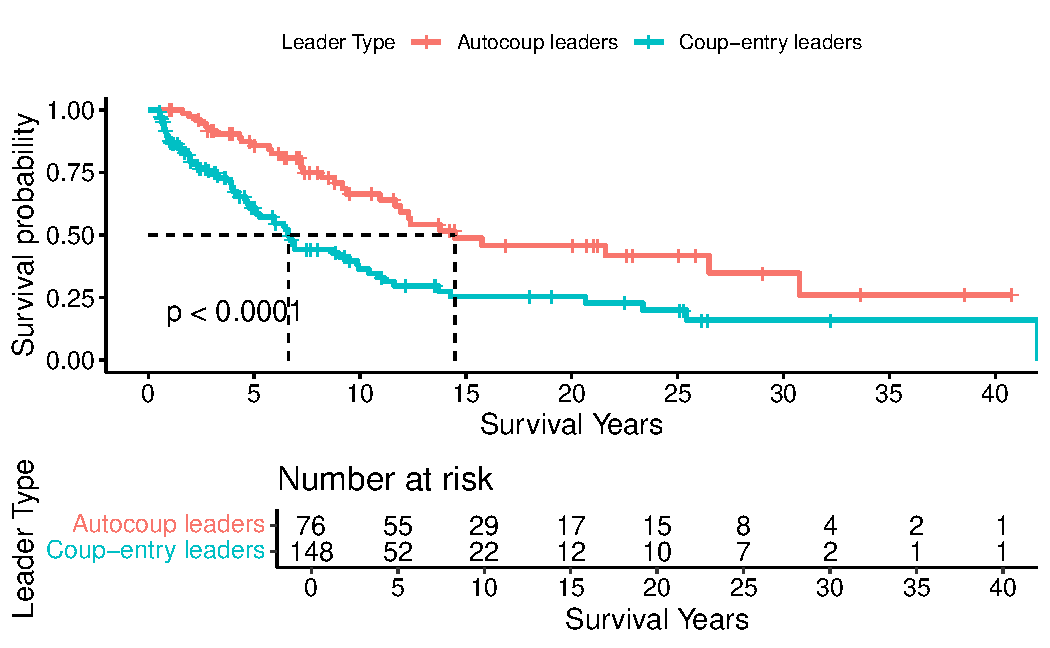
\includegraphics{_coups_and_autocoups_files/figure-pdf/fig-logrank-1.pdf}

}

\caption{\label{fig-logrank}Survival curves of overstaying and
coup-entry leaders}

\end{figure}%

A preliminary log-rank test in survival analysis, as illustrated in
Figure~\ref{fig-logrank}, demonstrates a statistically significant
difference between the tenures of autocoup and coup-entry leaders. The
survival curve for autocoup leaders consistently exceeds that of
coup-entry leaders, indicating longer survival times and a reduced risk
of ouster for autocoup leaders.

This study posits that the method of accession significantly influences
leadership longevity. Coup-entry leaders likely confront greater
challenges to their rule, resulting in shorter average tenures compared
to autocoup leaders. The analysis, employing Cox proportional hazards
and time-dependent Cox models, supports this hypothesis, demonstrating
that autocoup leaders generally experience longer tenures than
coup-entry leaders.

This research offers two primary contributions to the field. First, it
highlights an understudied factor in leadership survival analysis: the
impact of the method of accession to power. My findings suggest that
leader survival is influenced not only by ruling strategies but also by
the initial method of acquiring power. Second, by employing survival
models, this study provides empirical evidence of the significant
difference in tenure duration between autocoup and coup-entry leaders.
This insight may explain the increasing prevalence of tenure extensions
through autocoups since 2000, as more incumbents observe and potentially
emulate successful precedents.

The remainder of this chapter is structured as follows: Section 2
provides a comprehensive literature review on political survival,
establishing the context for this research. Section 3 explores the
factors influencing the survival of coup and autocoup leaders. Section 4
outlines the methodology and data used, including the application of
survival models to analyse the determinants of leadership longevity.
Section 5 presents the analysis findings and a detailed discussion of
the results. Finally, Section 6 concludes by synthesizing key takeaways
and exploring their broader implications for political stability and
democratic processes.

\section{Literature review}\label{literature-review}

The longevity of political leaders has been a central focus in political
science research for decades, driven by the wide-ranging variations
observed across regimes, countries, and historical periods. This field
encompasses two interconnected aspects: regime survival and individual
leader survival. Regime survival focuses on the endurance of political
systems, such as monarchies, political parties, or specific ideological
structures, while leader survival concerns the duration of individual
leaders' time in office.

These concepts often exhibit contrasting patterns. For instance,
parliamentary democracies like Japan or the United Kingdom may
experience prolonged periods of party dominance coupled with frequent
leadership changes, whereas communist regimes typically demonstrate
enduring party rule with more frequent leadership transitions.
Presidential systems, such as the United States or many military
regimes, tend to exhibit more frequent changes in both ruling party or
junta and leader. This study specifically investigates the dynamics of
individual leader survival, focusing on factors influencing the duration
of leaders' time in office.

The existing literature on leader survival is extensive and
multifaceted. Some studies explore specific mechanisms influencing
leadership longevity within particular regimes, such as democracies
(\citeproc{ref-svolik2014}{Svolik 2014}) or autocracies
(\citeproc{ref-davenport2021}{Davenport, RezaeeDaryakenari, and Wood
2021}), while others aim to develop more generalizable theoretical
frameworks explaining leader survival across different political systems
(\citeproc{ref-buenodemesquita2003}{Bueno de Mesquita et al. 2003}).
Although a universal theory remains an aspirational goal, the
complexities of leadership survival across diverse regime types present
significant challenges.

Power transition mechanisms vary substantially across different regimes,
particularly between democracies and autocracies. Autocratic systems
often feature closed leadership selection processes, restricted to a
narrow pool of individuals such as royal families, military elites, or
ruling party members. While some autocracies may hold elections,
significant barriers to entry for legitimate challengers typically
persist. Potential rivals may face threats like assassination,
imprisonment, or exile. Moreover, the opacity of selection processes
makes it difficult to assess genuine levels of public support compared
to democracies. Consequently, conceptualizing selectorates or winning
coalitions, as proposed by Bueno de Mesquita et al.
(\citeproc{ref-buenodemesquita2003}{2003}), becomes problematic in many
autocratic contexts.

Given these complexities, focusing research on specific regimes or
leader types may be more fruitful. While regular leadership changes
offer valuable insights, they provide limited opportunities to explore
the dynamics of leader survival. In contrast, the study of irregular
leaders, such as those who ascend to power through coups or overstay in
office through autocoups, offers a more compelling avenue for research
due to the inherent complexities and uncertainties surrounding their
leadership trajectories.

Two primary perspectives have emerged to explain the dynamics of leader
survival. The first emphasizes objective factors and resources, such as
personal competence (\citeproc{ref-yu2016}{Yu and Jong-A-Pin 2016}),
societal stability (\citeproc{ref-arriola2009}{Arriola 2009}), economic
development (\citeproc{ref-palmer1999}{Palmer and Whitten 1999};
\citeproc{ref-williams2011}{Williams 2011}), natural resource endowments
(\citeproc{ref-smith2004}{Smith 2004};
\citeproc{ref-quirozflores2012}{Quiroz Flores and Smith 2012};
\citeproc{ref-wright2013}{Wright, Frantz, and Geddes 2013}), and
external support (\citeproc{ref-licht2009}{Licht 2009};
\citeproc{ref-wright2008}{Wright 2008}; \citeproc{ref-thyne2017}{Thyne
et al. 2017}). The second focuses on subjective factors and strategies,
including political policies, responses to opposition, and tactics for
consolidating power (\citeproc{ref-gandhi2007}{Gandhi and Przeworski
2007}; \citeproc{ref-morrison2009}{Morrison 2009};
\citeproc{ref-escribuxe0-folch2013}{Escribà-Folch 2013};
\citeproc{ref-davenport2021}{Davenport, RezaeeDaryakenari, and Wood
2021}).

Coups have received considerable scholarly attention, with research
examining coup prevention strategies, the impact of coups on leadership,
and the subsequent actions of coup leaders. Existing research delves
into strategies for thwarting coups (\citeproc{ref-powell2017}{J. Powell
2017}; \citeproc{ref-sudduth2017}{Sudduth 2017};
\citeproc{ref-debruin2020}{De Bruin 2020}) and how leaders extend their
tenures after surviving coup attempts (\citeproc{ref-easton2018}{Easton
and Siverson 2018}). Sudduth (\citeproc{ref-sudduth2017}{2017}) examines
post-coup actions of dictators, focusing on purge strategies, while
Sudduth and Bell (\citeproc{ref-sudduth2018}{2018}) investigates how
leaders' entry methods affect their removal in dictatorships.

However, a significant gap exists in the literature regarding the
comparison of leadership survival between coup-entry and autocoup
leaders. This study aims to address this gap by investigating and
comparing the duration of leadership survival for these two leader
types, contributing to a more nuanced understanding of political
survival in irregular leadership transitions.

\section{Survival dynamics of autocoup and coup-entry
leaders}\label{survival-dynamics-of-autocoup-and-coup-entry-leaders}

The study of leadership survival in political systems presents inherent
challenges due to the opacity and diverse mechanisms of power
transitions. However, these challenges underscore the significance of
this research, as it illuminates understudied dynamics in political
leadership. While the survival of political leaders exhibits complexity
and variation, it is not entirely devoid of patterns. Leaders of similar
types often display significant comparability.

\subsection{Key Definitions and Scope}\label{key-definitions-and-scope}

Before delving into the comparison, it is essential to clarify several
key terminologies:

\begin{itemize}
\item
  \textbf{Coup and Autocoup}: These terms adhere to the definitions
  established in previous chapters.
\item
  \textbf{Tenure Length Threshold}: To ensure meaningful analysis, this
  study focuses on leaders with substantial periods in power, applying a
  six-month threshold to both autocoup and coup-entry leaders.
\item
  \textbf{Autocoup Leader}: An incumbent leader who successfully uses
  illegitimate or unconstitutional means to extend their tenure in
  power.
\item
  \textbf{Coup-Entry Leader}: The individual who assumes power after a
  successful coup, regardless of their role in the coup itself.
\end{itemize}

This study focuses on comparing the post-autocoup tenure of autocoup
leaders with the post-coup tenure of coup-entry leaders, motivated by
the relevance and similarity of these leader types in terms of
illegitimacy, uncertainty, and instability.

\subsection{Challenges in Power
Consolidation}\label{challenges-in-power-consolidation}

Both autocoup and coup-entry leaders face distinct challenges in
consolidating their power, primarily due to differences in the intensity
of issues related to illegitimacy, uncertainty, and instability. This
disparity creates an uneven playing field in terms of power dynamics,
with coup-entry leaders at a significant disadvantage.
Table~\ref{tbl-leaders} compares the main features between autocoup and
coup-entry leaders.

\blandscape

\begin{table}

\caption{\label{tbl-leaders}Main features of autocoup and coup-entry
leaders}

\centering{

\fontsize{12.0pt}{14.4pt}\selectfont
\begin{tabular*}{1\linewidth}{@{\extracolsep{\fill}}>{\raggedright\arraybackslash}p{\dimexpr 112.50pt -2\tabcolsep-1.5\arrayrulewidth}>{\raggedright\arraybackslash}p{\dimexpr 225.00pt -2\tabcolsep-1.5\arrayrulewidth}>{\raggedright\arraybackslash}p{\dimexpr 225.00pt -2\tabcolsep-1.5\arrayrulewidth}}
\toprule
Feature & Autocoup Leader & Coup Entry Leader \\ 
\midrule\addlinespace[2.5pt]
Illegitimacy & Normally attained through
lawful procedures, but
lacking consensus
legitimacy & Blatantly illegal \\ 
Uncertainty & Initially with some certainty, but decreases as the leader's age grows or health worsens & Significant uncertainty initially \\ 
Instability & Relatively stable & Unstable except when a strongman emerges or constitutional institutions are established \\ 
Balance of Power & Generally in a better position of power & Initially unclear and challenging to establish a balance \\ 
\bottomrule
\end{tabular*}

}

\end{table}%

\elandscape

\subsubsection*{Illegitimacy}\label{illegitimacy}
\addcontentsline{toc}{subsubsection}{Illegitimacy}

While both types of leaders suffer from a legitimacy deficit, the nature
of this deficit differs:

\begin{itemize}
\item
  \textbf{Coup-Entry Leaders}: Their illegitimacy is explicit due to the
  open seizure of power.
\item
  \textbf{Autocoup Leaders}: They employ a deceptive strategy,
  manipulating legal processes to create a façade of democratic
  legitimacy.
\end{itemize}

\subsubsection*{Uncertainty}\label{uncertainty}
\addcontentsline{toc}{subsubsection}{Uncertainty}

The irregular paths to power create uncertainty regarding their reigns
and eventual departures. However, the levels of uncertainty differ.

Coup-entry leaders face three major uncertainties: Unclear who will
assume leadership after the coup, uncertain tenure length, and ambiguity
regarding future successors.

Autocoup leaders present a clearer picture: No ambiguity about who will
rule after an autocoup, many seek to extend their rule indefinitely or
incrementally.

\subsubsection*{Instability}\label{instability}
\addcontentsline{toc}{subsubsection}{Instability}

The awareness of shaky legitimacy and persistent uncertainty breeds
insecurity and a sense of crisis.

Coup-entry leaders must reshape power dynamics and often purge potential
adversaries. They need to create a new equilibrium, often disrupting
established structures. They also face potential backlash even from
close allies and hence must compromise with internal or external power
challengers.

Autocoup leaders encounter fewer abrupt changes in their regimes. They
face less pressure to dismantle existing ruling paradigms and have more
time to implement changes gradually.

\subsection{Empirical Evidence and
Hypothesis}\label{empirical-evidence-and-hypothesis}

Empirical evidence supports the disadvantage faced by coup-entry
leaders. Data reveals a correlation between the frequency of coup
attempts in a country and the likelihood of future coups. Over a third
of coups occur in the top ten countries with the most attempts since
1950 (Table~\ref{tbl-coups}). The average survival period following an
autocoup is approximately five years longer than that of coup-entry
leaders (Figure~\ref{fig-logrank}).

The distinct challenges faced by autocoup and coup-entry leaders in
consolidating power create a self-perpetuating cycle that influences
their tenure length. Coup-entry leaders, facing greater challenges,
struggle to attract and retain strong support, making them more
vulnerable to internal and external challenges. Conversely, autocoup
leaders, often benefiting from a veneer of legitimacy and a stronger
initial position, are better able to consolidate power and attract
supporters, leading to potentially longer tenures.

Based on these observations, I propose the following hypothesis:

\textbf{\emph{H4-1: Political leaders who successfully extend their
tenure through autocoups are more likely to survive longer compared to
coup-entry leaders.}}

\section{Research Design}\label{research-design-1}

This study employs survival analysis to test the hypothesis that
autocoup leaders have longer survival times in office compared to
coup-entry leaders. The research design utilizes Cox models to analyze
the survival tenures of these two types of leaders, accounting for
multiple factors that may influence their time in power.

\subsection{Methodology: Survival
analysis}\label{methodology-survival-analysis}

Two Cox models will be employed to analyze the survival tenures of
coup-entry and autocoup leaders:

\begin{itemize}
\item
  \textbf{Cox Proportional Hazards (PH) Model}: This model uses only the
  variables present at the entry year, without considering changes over
  time.
\item
  \textbf{Time-Dependent Cox Model}: This model accounts for variations
  in time-dependent control variables such as economic performance and
  political stability.
\end{itemize}

The Cox model is preferred over the Kaplan-Meier model as it allows for
the estimation of multiple factors' impacts. While it does not directly
estimate the duration of tenure in office, it evaluates the hazard rate
associated with being ousted from power. This approach captures
different facets of the same phenomenon: as a leader's cumulative hazard
of being ousted increases, their probability of survival in office
decreases.

\subsection{Data and Variables}\label{data-and-variables}

The dependent variables include survival time and end point status:

\begin{itemize}
\item
  \textbf{Survival Time:} The duration of a leader's tenure, measured in
  days. For coup-entry leaders, the survival time begins on the day they
  assume power through a coup. For autocoup leaders, the survival time
  starts on the expiration date of their original legitimate term. For
  example, Xi Jinping assumed power in 2013 and removed term limits in
  2018. His original legitimate tenure was set to end in 2023, so his
  survival time begins in 2023, marking the start of his post-autocoup
  tenure. The survival time concludes on the day the leader exits
  office, applicable to both coup-entry and autocoup leaders.
\item
  \textbf{End point status:} This variable indicates the manner in which
  the leader's tenure concluded, categorized as follows:

  \textbf{0 = Censored:} This status is assigned to leaders who leave
  office through regular means other than being ousted. This includes
  leaders transferring power to their designated successors, leaving
  office as their terms expire, losing in general elections, voluntarily
  leaving office due to health issues, or dying of natural causes.

  \textbf{1 = Ousted:} This status is assigned to leaders who are forced
  to leave office. This includes leaders resigning under pressure, being
  ousted by coups or other forces, or being assassinated.
\end{itemize}

The key independent variable is the leader type, which categorizes
leaders into two distinct groups:

\begin{itemize}
\tightlist
\item
  \textbf{Group A = Autocoup Leader}: Leaders who extend their tenure
  through autocoups.
\item
  \textbf{Group B = Coup-Entry Leader}: Leaders who assume power through
  coups.
\end{itemize}

This variable is the primary independent variable of interest, serving
as the basis for comparing the survival time between these two types of
leaders.

The data for both dependent and independent variables are sourced from
the autocoup dataset introduced in this study, Archigos, and PLAD.

Control variables include economic performance, political stability,
population size, and the leader's age, which are consistent with the
autocoup analysis in Chapter~\ref{sec-chapter3}.

\section{Results and discussion}\label{results-and-discussion-1}

\subsection{Model results}\label{model-results}

Using the \texttt{survival} package in R
(\citeproc{ref-survival}{Therneau 2024}), I present the regression
results for both the Cox Proportional Hazards (Cox PH) model and the
time-dependent Cox model in Table~\ref{tbl-cox}.

\begin{table}

\caption{\label{tbl-cox}Cox models for survival time of different types
of leaders}

\centering{

\fontsize{12.0pt}{14.4pt}\selectfont
\begin{tabular*}{\linewidth}{@{\extracolsep{\fill}}lcccccccc}
\toprule
 & \multicolumn{4}{c}{\textbf{Cox PH Model}} & \multicolumn{4}{c}{\textbf{Time-dependent Cox Model}} \\ 
\cmidrule(lr){2-5} \cmidrule(lr){6-9}
\textbf{Characteristic} & \textbf{N} & \textbf{Event N} & \textbf{HR}\textsuperscript{\textit{1,2}} & \textbf{SE}\textsuperscript{\textit{2}} & \textbf{N} & \textbf{Event N} & \textbf{HR}\textsuperscript{\textit{1,2}} & \textbf{SE}\textsuperscript{\textit{2}} \\ 
\midrule\addlinespace[2.5pt]
{\bfseries Leader Type} &  &  &  &  &  &  &  &  \\ 
    Autocoup leaders & 76 & 31 & 1.00 & — & 737 & 29 & 1.00 & — \\ 
    Coup-entry leaders & 148 & 73 & 2.71*** & 0.252 & 853 & 73 & 2.23*** & 0.246 \\ 
{\bfseries GDP Growth Trend} & 224 & 104 & 1.95 & 1.08 & 1,590 & 102 & 0.20* & 0.981 \\ 
{\bfseries GDP per capita} & 224 & 104 & 0.97* & 0.020 & 1,590 & 102 & 0.95** & 0.023 \\ 
{\bfseries Population: log} & 224 & 104 & 0.98 & 0.083 & 1,590 & 102 & 0.90 & 0.079 \\ 
{\bfseries Polity 5} & 224 & 104 & 0.99 & 0.025 & 1,590 & 102 & 1.01 & 0.023 \\ 
{\bfseries Political stability} & 224 & 104 & 1.00 & 0.053 & 1,590 & 102 & 1.11* & 0.049 \\ 
{\bfseries Age} & 224 & 104 & 1.01 & 0.010 & 1,590 & 102 & 1.00 & 0.011 \\ 
\bottomrule
\end{tabular*}
\begin{minipage}{\linewidth}
\textsuperscript{\textit{1}}*p\textless{}0.1; **p\textless{}0.05; ***p\textless{}0.01\\
\textsuperscript{\textit{2}}HR = Hazard Ratio, SE = Standard Error\\
\end{minipage}

}

\end{table}%

Both the Cox PH model and the time-dependent Cox model analyses revealed
a statistically significant association between leadership type and the
hazard of removal from power. Since time-dependent Cox model use the
control variables which change over time, I interpret the main findings
based on time-dependent model.

Coup-entry leaders were found to have a hazard ratio of 2.23 in the
time-dependent model compared to autocoup leaders (reference group),
assuming all other variables in the model are held constant. This
suggests that coup-entry leaders face a significantly greater risk of
removal from power compared to autocoup leaders. At any given time
during their tenure, coup-entry leaders are 2.23 times more likely to be
ousted from power compared to autocoup leaders, all else being equal in
the model.

The control variables perform differently in the two models. Economic
level (GDP per capita) exhibits statistically significant effects in
both models. In the time-dependent model, the hazard ratio of 0.95
indicates that for each unit increase in GDP per capita (measured in
units of \$10,000), the hazard (or risk) of being ousted at any given
time is reduced by 5\%, assuming all other variables in the model are
held constant.

GDP growth trend demonstrates a more substantial effect in reducing the
risk of coups. Specifically, a 1 percentage point higher economic growth
trend is associated with an 80\% reduction in the risk of being ousted,
although this effect is only statistically significant at the 10\%
level. This suggests a possible trend where positive economic
performance might mitigate the risk of removal from power, but the
evidence is not robust enough to confirm this conclusively.

Political stability, as measured by the violence index, shows that a
1-point increase in the index correlates with an 11\% higher risk of
being ousted. However, this effect is also only statistically
significant at the 10\% level, indicating a weaker but potentially
important relationship between increased violence and the risk of
removal from office.

\subsection{Discussion}\label{discussion}

\begin{figure}

\begin{minipage}{0.50\linewidth}

\centering{

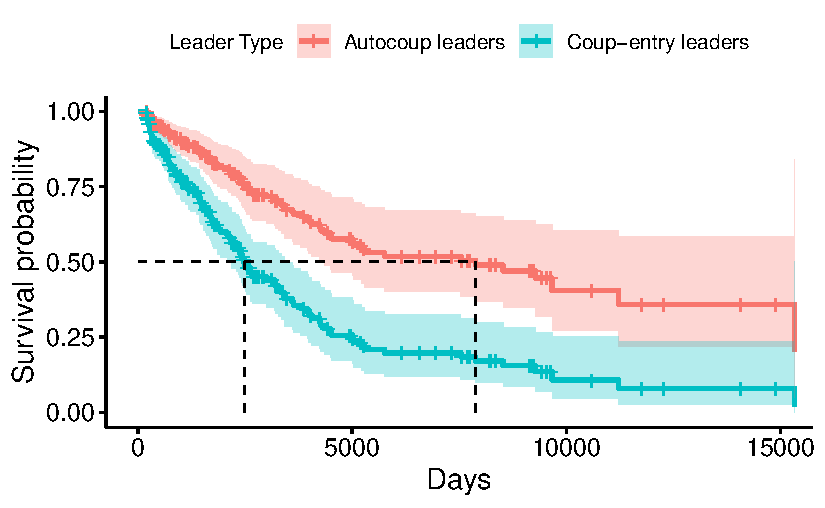
\includegraphics{_coups_and_autocoups_files/figure-pdf/fig-coxSurv-1.pdf}

}

\subcaption{\label{fig-coxSurv-1}Cox PH Model}

\end{minipage}%
%
\begin{minipage}{0.50\linewidth}

\centering{

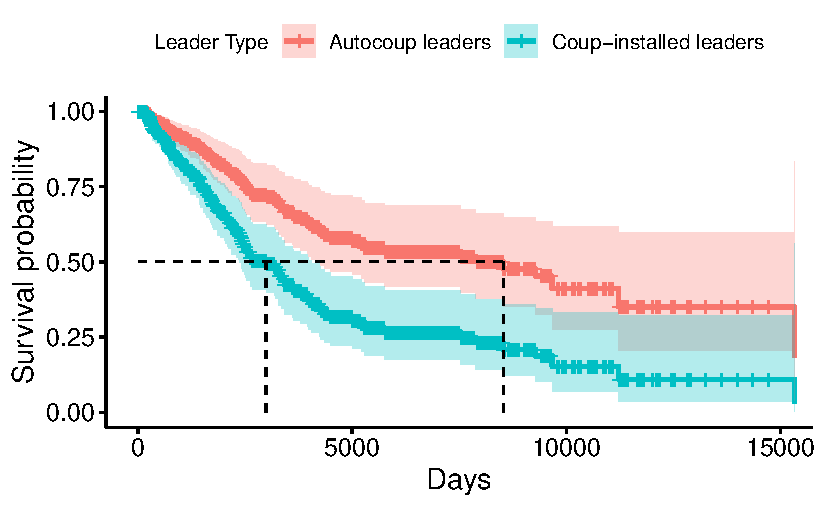
\includegraphics{_coups_and_autocoups_files/figure-pdf/fig-coxSurv-2.pdf}

}

\subcaption{\label{fig-coxSurv-2}Time-dependent Cox Model}

\end{minipage}%

\caption{\label{fig-coxSurv}Survival curves for Cox Model}

\end{figure}%

The survival curves depicted in Figure~\ref{fig-coxSurv} illustrate the
survival rates for leaders of both types. Both the Cox PH model and the
time-dependent Cox model produce similar plots. Notably, the survival
curve for coup-entry leaders exhibits a significantly lower trajectory
compared to that of autocoup leaders. The steeper drop at the early
stage for coup-entry leaders indicates they are more likely to be ousted
shortly after assuming power. Additionally, the survival curve for
coup-entry leaders crosses the median survival line much earlier (about
3,000 days) than that of autocoup leaders (about 8,500 days). This
disparity suggests that autocoup leaders tend to remain in power for
longer durations than their coup-entry counterparts.

\begin{figure}

\begin{minipage}{0.50\linewidth}

\centering{

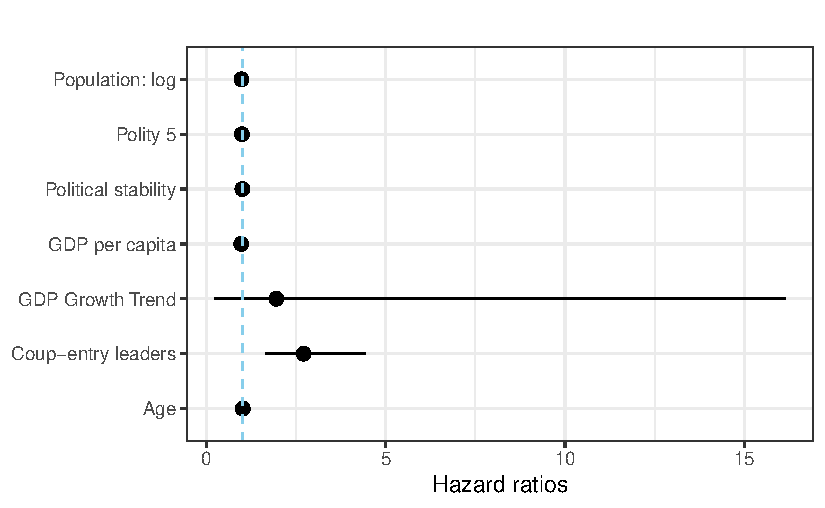
\includegraphics{_coups_and_autocoups_files/figure-pdf/fig-coxHR-1.pdf}

}

\subcaption{\label{fig-coxHR-1}Cox PH Model}

\end{minipage}%
%
\begin{minipage}{0.50\linewidth}

\centering{

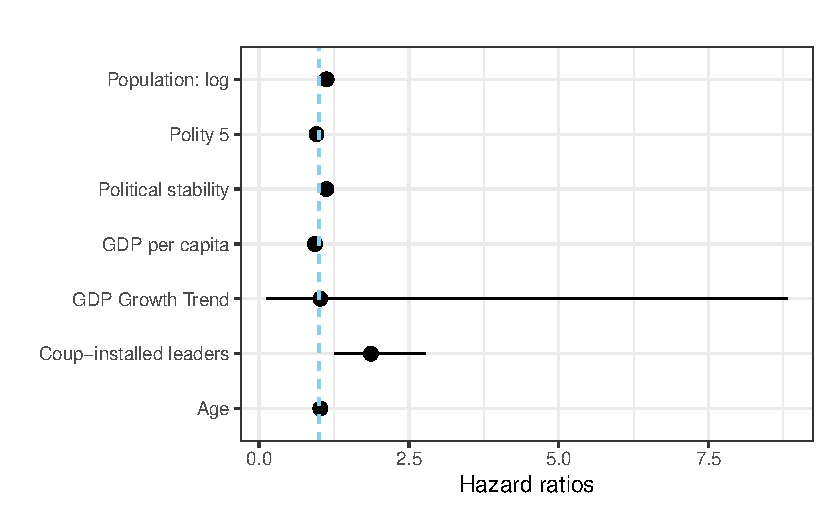
\includegraphics{_coups_and_autocoups_files/figure-pdf/fig-coxHR-2.pdf}

}

\subcaption{\label{fig-coxHR-2}Time-dependent Cox Model}

\end{minipage}%

\caption{\label{fig-coxHR}Hazard ratios and 95\% CIs for Leader Ousting}

\end{figure}%

Figure~\ref{fig-coxHR} displays the hazard ratios and corresponding 95\%
confidence intervals for the variables incorporated in the Cox model.
Both the Cox Proportional Hazards (PH) model and the time-dependent
model produce similar plots, reinforcing the robustness of the findings.
Key points to note include:

\begin{itemize}
\item
  The closer the hazard ratio (represented by the dots) is to 1, the
  less impact the variable has on the risk of being ousted. A hazard
  ratio of 1 indicates no effect.
\item
  The whiskers extending from the dots represent the 95\% confidence
  intervals. If these whiskers cross the vertical blue line at 1, it
  indicates that the variable is not statistically significant at the
  5\% level.
\item
  The hazard ratio for coup-entry leaders is significantly greater than
  1 and statistically significant at the 5\% level. This indicates that
  coup-entry leaders face a substantially higher risk of being ousted
  compared to autocoup leaders.
\item
  Most other variables have hazard ratios close to 1, suggesting that a
  one-unit increase in these variables does not significantly affect the
  risk of being ousted.
\item
  Although the hazard ratio for GDP growth trend is considerably less
  than 1 in the time-dependent model, indicating a potential protective
  effect, it is not statistically significant at the 5\% level. However,
  it is statistically significant at the 10\% level, suggesting that
  better economic performance may help to consolidate the rule of the
  incumbents to some extent, albeit the evidence is not as strong.
\end{itemize}

\subsection{Assessing the Proportional Hazards
Assumption}\label{assessing-the-proportional-hazards-assumption}

Assessing the proportional hazards assumption is crucial for the
validity of the Cox model results. To evaluate this, we used the
chi-square test based on Schoenfeld residuals to determine whether the
covariate effects remain constant (proportional) over time. Although the
Cox PH model violates the proportional hazards assumption, our primary
analysis relies on the time-dependent Cox model, which does not show
strong evidence of violating the proportional hazards assumption for any
covariate. The global p-value of 0.416 is much greater than the 5\%
significance level, indicating that the proportional hazards assumption
is reasonably met for the time-dependent Cox model.

\section{Conclusion}\label{conclusion-2}

This chapter examined the survival durations of political leaders who
come to power through irregular means, specifically coups and autocoups.
I hypothesized that the mode of accession significantly influences
leader tenure. Employing survival analysis techniques, including the Cox
proportional hazards model and a time-dependent Cox model, I found
strong evidence that autocoup leaders generally enjoy longer tenures
than coup-entry leaders.

The findings revealed a significant difference in average tenure, with
post-autocoup leaders averaging approximately 11 years in power compared
to 5.6 years for coup-entry leaders. The time-dependent Cox model
further indicated that coup-entry leaders are 2.23 times more likely to
be ousted from power at any given time compared to autocoup leaders, all
else being equal.

These results highlight the importance of understanding the phenomenon
of autocoups, where leaders extend their rule by manipulating legal
frameworks. Due to the relative ease and potential benefits of
autocoups, this method of power retention might incentivize more leaders
to employ it. Consequently, democratic backsliding could become more
prevalent as autocoups weaken democratic institutions and constitutional
norms, particularly in nascent democracies or those transitioning from
autocracy.

This study contributes to the field of leadership survival by
demonstrating that the mode of accession significantly impacts leader
tenure, a factor previously under-explored in the literature. By
utilizing both Cox models, the research offers robust analytical
techniques for studying political leadership survival and provides
strong evidence of divergent tenure lengths between these two types of
irregular-entry leaders.

However, limitations exist. The study relies heavily on the autocoup
dataset collected and coded by the author. The concept and data itself
are relatively novel within academia. Future research should refine and
establish wider recognition for the term ``autocoup,'' leading to more
accurate and comprehensive data collection efforts. Expanding the
dataset to include more cases and integrating it with data on other
irregular leadership transitions could yield a more holistic
understanding of political survival in such contexts.

Overall, this chapter underscores the need for more nuanced approaches
to studying political tenure and the mechanisms of irregular power
retention, contributing valuable insights into the dynamics of political
stability and the risks associated with different forms of
non-democratic leadership succession.

\chapter{Conclusion}\label{conclusion-3}

\section{Main Findings}\label{main-findings}

This study delves into the dynamics and implications of irregular power
transitions, focusing on coups and autocoups. The findings illuminate
the complex interplay between incumbents and challengers fighting for
power.

Firstly, our analysis reveals that the expected success rate of a coup
attempt significantly influences its likelihood. This success rate is
heavily influenced by the balance of power between the incumbent regime
and challengers, which is largely determined by regime type. We find
that military regimes, although with more control over their own
military forces, face a higher risk of coups compared to dominant-party
regimes.

Secondly, the study introduces a redefined concept: the autocoup.
Defined as an incumbent leader's refusal to relinquish power as
mandated, this research distinguishes autocoups from broader terms like
self-coups. Based on this definition, we present the first publicly
available dataset of autocoup events from 1945 to 2022, encompassing 110
attempts and 87 successful autocoups. Case studies and empirical
analyses demonstrate the dataset's utility for quantitative research,
providing a robust foundation for further analysis on autocoups.

Thirdly, employing survival analysis techniques, the study finds clear
differences in leader longevity between those who come to power through
coups and those who extend their rule through autocoups. The results
indicate that coup-installed leaders face a significantly higher risk of
removal compared to autocoup leaders who manipulate the system to extend
their rule.

\section{Limitations and directions for future
research}\label{limitations-and-directions-for-future-research}

This study offers a novel framework for analysing irregular power
transitions, but some limitations require further exploration:

\begin{itemize}
\item
  \textbf{Data refinement:} Defining and classifying autocoups is a new
  approach. Future research should validate this classification system
  through additional studies and expert evaluations.
\item
  \textbf{Data harmonization:} The current analysis faces challenges due
  to mismatched units (country-year vs.~leader) between coup and
  autocoup datasets. Future efforts should explore data harmonization
  techniques for more robust comparisons.
\item
  \textbf{Democratic backsliding:} While this study establishes a
  connection between irregular power transitions and democratic
  backsliding, further empirical evidence is needed to solidify this
  link.
\end{itemize}

Several avenues exist for future research:

\begin{itemize}
\item
  \textbf{Terminology and data collection:} Refining the ``autocoup''
  concept and achieving wider recognition will facilitate more accurate
  and comprehensive data collection.
\item
  \textbf{Dataset expansion:} Expanding the autocoup dataset with more
  cases and integrating it with data on other irregular leadership
  transitions can provide a more holistic view of political survival
  after these events.
\item
  \textbf{Power dynamics and long-term impacts:} Utilizing this dataset,
  future studies can delve deeper into power dynamics at play and
  explore the long-term consequences of irregular transitions on
  political systems, particularly regarding democratic backsliding,
  breakdown, and personalization of power.
\end{itemize}

In conclusion, this study sheds light on the dynamics of irregular power
transitions, specifically focusing on coups and autocoups. By redefining
autocoups, classifying the dataset, analysing determinants, and
comparing leader longevity, we establish a framework for understanding
irregular transitions and leader survival. This work contributes to a
deeper understanding of democratic resilience and political stability.
Future research can build upon this foundation by conducting further
empirical analyses based on the novel autocoup dataset and continuing to
refine the framework.

\newpage

\chapter*{References}\label{references}
\addcontentsline{toc}{chapter}{References}

\phantomsection\label{refs}
\begin{CSLReferences}{1}{0}
\bibitem[\citeproctext]{ref-aidt2019}
Aidt, Toke, and Gabriel Leon. 2019. {``The Coup.''} Edited by Roger D.
Congleton, Bernard Grofman, and Stefan Voigt, February.
\url{https://doi.org/10.1093/oxfordhb/9780190469771.013.15}.

\bibitem[\citeproctext]{ref-antonio2021}
Antonio, Robert J. 2021. {``Democracy and Capitalism in the Interregnum:
Trump{'}s Failed Self-Coup and After.''} \emph{Critical Sociology} 48
(6): 937--65. \url{https://doi.org/10.1177/08969205211049499}.

\bibitem[\citeproctext]{ref-arriola2009}
Arriola, Leonardo R. 2009. {``Patronage and Political Stability in
Africa.''} \emph{Comparative Political Studies} 42 (10): 1339--62.
\url{https://doi.org/10.1177/0010414009332126}.

\bibitem[\citeproctext]{ref-baturo2014}
Baturo, Alexander. 2014. {``Democracy, Dictatorship, and Term Limits.''}
\url{https://doi.org/10.3998/mpub.4772634}.

\bibitem[\citeproctext]{ref-baturo2019}
---------. 2019. {``Continuismo in Comparison.''} In, 75--100. Oxford
University Press.
\url{https://doi.org/10.1093/oso/9780198837404.003.0005}.

\bibitem[\citeproctext]{ref-baturo2022}
Baturo, Alexander, and Jakob Tolstrup. 2022. {``Incumbent Takeovers.''}
\emph{Journal of Peace Research} 60 (2): 373--86.
\url{https://doi.org/10.1177/00223433221075183}.

\bibitem[\citeproctext]{ref-bermeo2016}
Bermeo, Nancy. 2016. {``On Democratic Backsliding.''} \emph{Journal of
Democracy} 27 (1): 5--19. \url{https://doi.org/10.1353/jod.2016.0012}.

\bibitem[\citeproctext]{ref-buxf6hmelt2014}
Böhmelt, Tobias, and Ulrich Pilster. 2014. {``The Impact of
Institutional Coup-Proofing on Coup Attempts and Coup Outcomes.''}
\emph{International Interactions} 41 (1): 158--82.
\url{https://doi.org/10.1080/03050629.2014.906411}.

\bibitem[\citeproctext]{ref-bomprezzi2024wedded}
Bomprezzi, Pietro, Axel Dreher, Andreas Fuchs, Teresa Hailer, Andreas
Kammerlander, Lennart Kaplan, Silvia Marchesi, Tania Masi, Charlotte
Robert, and Kerstin Unfried. 2024. {``Wedded to Prosperity? Informal
Influence and Regional Favoritism.''} Discussion Paper. CEPR.

\bibitem[\citeproctext]{ref-brown2001}
Brown, Stephen. 2001. {``Authoritarian Leaders and Multiparty Elections
in Africa: How Foreign Donors Help to Keep Kenya's Daniel Arap Moi in
Power.''} \emph{Third World Quarterly} 22 (5): 725--39.
\url{https://doi.org/10.1080/01436590120084575}.

\bibitem[\citeproctext]{ref-buenodemesquita2003}
Bueno de Mesquita, Bruce, Alastair Smith, Randolph M. Siverson, and
James D. Morrow. 2003. \emph{The Logic of Political Survival}. The MIT
Press. \url{https://doi.org/10.7551/mitpress/4292.001.0001}.

\bibitem[\citeproctext]{ref-cameron1998a}
Cameron, Maxwell A. 1998a. {``Latin American Autogolpes : Dangerous
Undertows in the Third Wave of Democratisation.''} \emph{Third World
Quarterly} 19 (2): 219--39.
\url{https://doi.org/10.1080/01436599814433}.

\bibitem[\citeproctext]{ref-cameron1998}
Cameron, Maxwell A. 1998b. {``Self-Coups: Peru, Guatemala, and
Russia.''} \emph{Journal of Democracy} 9 (1): 125--39.
\url{https://doi.org/10.1353/jod.1998.0003}.

\bibitem[\citeproctext]{ref-cassani2020}
Cassani, Andrea. 2020. {``Autocratisation by Term Limits Manipulation in
Sub-Saharan Africa.''} \emph{Africa Spectrum} 55 (3): 228--50.
\url{https://doi.org/10.1177/0002039720964218}.

\bibitem[\citeproctext]{ref-cheeseman2015}
Cheeseman, Nic. 2015. {``Democracy in Africa,''} March.
\url{https://doi.org/10.1017/cbo9781139030892}.

\bibitem[\citeproctext]{ref-cheeseman2019}
---------. 2019. {``Should I Stay or Should I Go? Term Limits,
Elections, and Political Change in Kenya, Uganda, and Zambia.''} In,
311--38. Oxford University PressOxford.
\url{https://doi.org/10.1093/oso/9780198837404.003.0016}.

\bibitem[\citeproctext]{ref-cheeseman2019a}
Cheeseman, Nic, and Brian Klaas. 2019. \emph{How to Rig an Election}.
Yale University Press. \url{https://doi.org/10.12987/9780300235210}.

\bibitem[\citeproctext]{ref-choulis2022}
Choulis, Ioannis, Marius Mehrl, Abel Escribà-Folch, and Tobias Böhmelt.
2022. {``How Mechanization Shapes Coups.''} \emph{Comparative Political
Studies} 56 (2): 267--96.
\url{https://doi.org/10.1177/00104140221100194}.

\bibitem[\citeproctext]{ref-close2019}
Close, David. 2019. {``Presidential Term Limits in Nicaragua.''} In,
159--78. Oxford University PressOxford.
\url{https://doi.org/10.1093/oso/9780198837404.003.0009}.

\bibitem[\citeproctext]{ref-davenport2021}
Davenport, Christian, Babak RezaeeDaryakenari, and Reed M Wood. 2021.
{``Tenure Through Tyranny? Repression, Dissent, and Leader Removal in
Africa and Latin America, 1990{\textendash}2006.''} \emph{Journal of
Global Security Studies} 7 (1).
\url{https://doi.org/10.1093/jogss/ogab023}.

\bibitem[\citeproctext]{ref-debruin2020}
De Bruin, Erica. 2020. {``Preventing Coups d{'}état.''} In, 1--12.
Cornell University Press.
\url{https://doi.org/10.7591/cornell/9781501751912.003.0001}.

\bibitem[\citeproctext]{ref-easton2018}
Easton, Malcolm R, and Randolph M Siverson. 2018. {``Leader Survival and
Purges After a Failed Coup d{'}état.''} \emph{Journal of Peace Research}
55 (5): 596--608. \url{https://doi.org/10.1177/0022343318763713}.

\bibitem[\citeproctext]{ref-escribuxe0-folch2013}
Escribà-Folch, Abel. 2013. {``Repression, Political Threats, and
Survival Under Autocracy.''} \emph{International Political Science
Review} 34 (5): 543--60. \url{https://doi.org/10.1177/0192512113488259}.

\bibitem[\citeproctext]{ref-ezrow2019}
Ezrow, Natasha. 2019. {``Term Limits and Succession in Dictatorships.''}
In, 269--88. Oxford University PressOxford.
\url{https://doi.org/10.1093/oso/9780198837404.003.0014}.

\bibitem[\citeproctext]{ref-fariss2022}
Fariss, Christopher J., Therese Anders, Jonathan N. Markowitz, and
Miriam Barnum. 2022. {``New Estimates of Over 500 Years of Historic GDP
and Population Data.''} \emph{Journal of Conflict Resolution} 66 (3):
553--91. \url{https://doi.org/10.1177/00220027211054432}.

\bibitem[\citeproctext]{ref-frantz2016}
Frantz, Erica, and Elizabeth A. Stein. 2016. {``Countering Coups:
Leadership Succession Rules in Dictatorships.''} \emph{Comparative
Political Studies} 50 (7): 935--62.
\url{https://doi.org/10.1177/0010414016655538}.

\bibitem[\citeproctext]{ref-freedomhouse2024freedom}
Freedom House. 2024. {``Freedom in the World 2024.''}
\url{https://freedomhouse.org/sites/default/files/2024-02/FIW_2024_DigitalBooklet.pdf}.

\bibitem[\citeproctext]{ref-gandhi2007}
Gandhi, Jennifer, and Adam Przeworski. 2007. {``Authoritarian
Institutions and the Survival of Autocrats.''} \emph{Comparative
Political Studies} 40 (11): 1279--1301.
\url{https://doi.org/10.1177/0010414007305817}.

\bibitem[\citeproctext]{ref-gassebner2016}
Gassebner, Martin, Jerg Gutmann, and Stefan Voigt. 2016. {``When to
Expect a Coup d{'}état? An Extreme Bounds Analysis of Coup
Determinants.''} \emph{Public Choice} 169 (3-4): 293--313.
\url{https://doi.org/10.1007/s11127-016-0365-0}.

\bibitem[\citeproctext]{ref-geddes1999}
Geddes, Barbara. 1999. {``What Do We Know About Democratization After
Twenty Years?''} \emph{Annual Review of Political Science} 2 (1):
115--44. \url{https://doi.org/10.1146/annurev.polisci.2.1.115}.

\bibitem[\citeproctext]{ref-geddes2014}
Geddes, Barbara, Joseph Wright, and Erica Frantz. 2014. {``Autocratic
Breakdown and Regime Transitions: A New Data Set.''} \emph{Perspectives
on Politics} 12 (2): 313--31.
\url{https://doi.org/10.1017/s1537592714000851}.

\bibitem[\citeproctext]{ref-ginsburg2019}
Ginsburg, Tom, and Zachary Elkins. 2019. {``One Size Does Not Fit
All.''} In, 37--52. Oxford University Press.
\url{https://doi.org/10.1093/oso/9780198837404.003.0003}.

\bibitem[\citeproctext]{ref-ginsburg2010evasion}
Ginsburg, Tom, James Melton, and Zachary Elkins. 2010. {``On the Evasion
of Executive Term Limits.''} \emph{Wm. \& Mary L. Rev.} 52: 1807.

\bibitem[\citeproctext]{ref-ginsburg2011evasion}
---------. 2011. {``On the Evasion of Executive Term Limits.''}
\emph{William and Mary Law Review} 52: 1807.

\bibitem[\citeproctext]{ref-goemans2009}
Goemans, Henk E., Kristian Skrede Gleditsch, and Giacomo Chiozza. 2009.
{``Introducing Archigos: A Dataset of Political Leaders.''}
\emph{Journal of Peace Research} 46 (2): 269--83.
\url{https://doi.org/10.1177/0022343308100719}.

\bibitem[\citeproctext]{ref-helmke2017}
Helmke, Gretchen. 2017. {``Institutions on the Edge,''} January.
\url{https://doi.org/10.1017/9781139031738}.

\bibitem[\citeproctext]{ref-klesner2019}
Klesner, Joseph L. 2019. {``The Politics of Presidential Term Limits in
Mexico.''} In, 141--58. Oxford University Press.
\url{https://doi.org/10.1093/oso/9780198837404.003.0008}.

\bibitem[\citeproctext]{ref-krishnarajan2019}
Krishnarajan, Suthan. 2019. {``Economic Crisis, Natural Resources, and
Irregular Leader Removal in Autocracies.''} \emph{International Studies
Quarterly} 63 (3): 726--41. \url{https://doi.org/10.1093/isq/sqz006}.

\bibitem[\citeproctext]{ref-landau2019}
Landau, David, Yaniv Roznai, and Rosalind Dixon. 2019. {``Term Limits
and the Unconstitutional Constitutional Amendment Doctrine.''} In,
53--74. Oxford University PressOxford.
\url{https://doi.org/10.1093/oso/9780198837404.003.0004}.

\bibitem[\citeproctext]{ref-licht2009}
Licht, Amanda A. 2009. {``Coming into Money: The Impact of Foreign Aid
on Leader Survival.''} \emph{Journal of Conflict Resolution} 54 (1):
58--87. \url{https://doi.org/10.1177/0022002709351104}.

\bibitem[\citeproctext]{ref-llanos2019}
Llanos, Mariana. 2019. {``The Politics of Presidential Term Limits in
Argentina.''} In, 473--94. Oxford University Press.
\url{https://doi.org/10.1093/oso/9780198837404.003.0023}.

\bibitem[\citeproctext]{ref-marshall2005current}
Marshall, Monty G. 2005. {``Current Status of the World's Major Episodes
of Political Violence.''} \emph{Report to Political Instability Task
Force.(3 February)}.

\bibitem[\citeproctext]{ref-marsteintredet2019a}
Marsteintredet, Leiv. 2019. {``Presidential Term Limits in Latin
America: {\emph{C}}.1820{\textendash}1985.''} In, 103--22. Oxford
University PressOxford.
\url{https://doi.org/10.1093/oso/9780198837404.003.0006}.

\bibitem[\citeproctext]{ref-marsteintredet2019}
Marsteintredet, Leiv, and Andrés Malamud. 2019. {``Coup with Adjectives:
Conceptual Stretching or Innovation in Comparative Research?''}
\emph{Political Studies} 68 (4): 1014--35.
\url{https://doi.org/10.1177/0032321719888857}.

\bibitem[\citeproctext]{ref-mauceri1995}
Mauceri, Philip. 1995. {``State Reform, Coalitions, and The Neoliberal
{\emph{Autogolpe}} in Peru.''} \emph{Latin American Research Review} 30
(1): 7--37. \url{https://doi.org/10.1017/s0023879100017155}.

\bibitem[\citeproctext]{ref-mechkova2017}
Mechkova, Valeriya, Anna Lührmann, and Staffan I. Lindberg. 2017. {``How
Much Democratic Backsliding?''} \emph{Journal of Democracy} 28 (4):
162--69. \url{https://doi.org/10.1353/jod.2017.0075}.

\bibitem[\citeproctext]{ref-morrison2009}
Morrison, Kevin M. 2009. {``Oil, Nontax Revenue, and the
Redistributional Foundations of Regime Stability.''} \emph{International
Organization} 63 (1): 107--38.
\url{https://doi.org/10.1017/s0020818309090043}.

\bibitem[\citeproctext]{ref-neto2019}
Neto, Octavio Amorim, and Igor P. Acácio. 2019. {``Presidential Term
Limits as a Credible-Commitment Mechanism.''} In, 123--40. Oxford
University PressOxford.
\url{https://doi.org/10.1093/oso/9780198837404.003.0007}.

\bibitem[\citeproctext]{ref-nurumov2019}
Nurumov, Dmitry, and Vasil Vashchanka. 2019. {``Presidential Terms in
Kazakhstan.''} In, 221--46. Oxford University PressOxford.
\url{https://doi.org/10.1093/oso/9780198837404.003.0012}.

\bibitem[\citeproctext]{ref-palmer1999}
Palmer, Harvey D., and Guy D. Whitten. 1999. {``The Electoral Impact of
Unexpected Inflation and Economic Growth.''} \emph{British Journal of
Political Science} 29 (4): 623--39.
\url{https://doi.org/10.1017/s0007123499000307}.

\bibitem[\citeproctext]{ref-pion-berlin2022}
Pion-Berlin, David, Thomas Bruneau, and Richard B. Goetze. 2022. {``The
Trump Self-Coup Attempt: Comparisons and Civil{\textendash}Military
Relations.''} \emph{Government and Opposition} 58 (4): 789--806.
\url{https://doi.org/10.1017/gov.2022.13}.

\bibitem[\citeproctext]{ref-posner}
Posner, Daniel N., and Daniel J. Young. n.d. {``Term Limits: Leadership,
Political Competition and the Transfer of Power.''} In, 260--78.
Cambridge University Press.
\url{https://doi.org/10.1017/9781316562888.011}.

\bibitem[\citeproctext]{ref-powell2012}
Powell, Jonathan. 2012. {``Determinants of the Attempting and Outcome of
Coups d{'}état.''} \emph{Journal of Conflict Resolution} 56 (6):
1017--40. \url{https://doi.org/10.1177/0022002712445732}.

\bibitem[\citeproctext]{ref-powell2017}
---------. 2017. {``Leader Survival Strategies and the Onset of Civil
Conflict: A Coup-Proofing Paradox.''} \emph{Armed Forces \& Society} 45
(1): 27--44. \url{https://doi.org/10.1177/0095327x17728493}.

\bibitem[\citeproctext]{ref-powell2011}
Powell, Jonathan M, and Clayton L Thyne. 2011. {``Global Instances of
Coups from 1950 to 2010: A New Dataset.''} \emph{Journal of Peace
Research} 48 (2): 249--59.
\url{https://doi.org/10.1177/0022343310397436}.

\bibitem[\citeproctext]{ref-powell2018}
Powell, Jonathan, Christopher Faulkner, William Dean, and Kyle Romano.
2018. {``Give Them Toys? Military Allocations and Regime Stability in
Transitional Democracies.''} \emph{Democratization} 25 (7): 1153--72.
\url{https://doi.org/10.1080/13510347.2018.1450389}.

\bibitem[\citeproctext]{ref-przeworski2000}
Przeworski, Adam, Michael E. Alvarez, Jose Antonio Cheibub, and Fernando
Limongi. 2000. {``Democracy and Development,''} August.
\url{https://doi.org/10.1017/cbo9780511804946}.

\bibitem[\citeproctext]{ref-quirozflores2012}
Quiroz Flores, Alejandro, and Alastair Smith. 2012. {``Leader Survival
and Natural Disasters.''} \emph{British Journal of Political Science} 43
(4): 821--43. \url{https://doi.org/10.1017/s0007123412000609}.

\bibitem[\citeproctext]{ref-reyntjens2016}
Reyntjens, Filip. 2016. {``A New Look at the Evidence.''} \emph{Journal
of Democracy} 27 (3): 61--68.
\url{https://doi.org/10.1353/jod.2016.0044}.

\bibitem[\citeproctext]{ref-singh2016}
Singh, Naunihal. 2016. \emph{Seizing Power}. Johns Hopkins University
Press. \url{https://doi.org/10.1353/book.31450}.

\bibitem[\citeproctext]{ref-smith2004}
Smith, Benjamin. 2004. {``Oil Wealth and Regime Survival in the
Developing World, 1960{\textendash}1999.''} \emph{American Journal of
Political Science} 48 (2): 232--46.
\url{https://doi.org/10.1111/j.0092-5853.2004.00067.x}.

\bibitem[\citeproctext]{ref-stinnett2002}
Stinnett, Douglas M., Jaroslav Tir, Paul F. Diehl, Philip Schafer, and
Charles Gochman. 2002. {``The Correlates of War (Cow) Project Direct
Contiguity Data, Version 3.0.''} \emph{Conflict Management and Peace
Science} 19 (2): 59--67.
\url{https://doi.org/10.1177/073889420201900203}.

\bibitem[\citeproctext]{ref-sudduth2017}
Sudduth, Jun Koga. 2017. {``Strategic Logic of Elite Purges in
Dictatorships.''} \emph{Comparative Political Studies} 50 (13):
1768--1801. \url{https://doi.org/10.1177/0010414016688004}.

\bibitem[\citeproctext]{ref-sudduth2018}
Sudduth, Jun Koga, and Curtis Bell. 2018. {``The Rise Predicts the Fall:
How the Method of Leader Entry Affects the Method of Leader Removal in
Dictatorships.''} \emph{International Studies Quarterly} 62 (1):
145--59. \url{https://doi.org/10.1093/isq/sqx075}.

\bibitem[\citeproctext]{ref-svolik2014}
Svolik, Milan W. 2014. {``Which Democracies Will Last? Coups, Incumbent
Takeovers, and the Dynamic of Democratic Consolidation.''} \emph{British
Journal of Political Science} 45 (4): 715--38.
\url{https://doi.org/10.1017/s0007123413000550}.

\bibitem[\citeproctext]{ref-tangri2010}
Tangri, Roger, and Andrew M. Mwenda. 2010. {``President Museveni and the
Politics of Presidential Tenure in Uganda.''} \emph{Journal of
Contemporary African Studies} 28 (1): 31--49.
\url{https://doi.org/10.1080/02589000903542574}.

\bibitem[\citeproctext]{ref-survival}
Therneau, Terry M. 2024. {``A Package for Survival Analysis in r.''}
\url{https://CRAN.R-project.org/package=survival}.

\bibitem[\citeproctext]{ref-thyne2017}
Thyne, Clayton, Jonathan Powell, Sarah Parrott, and Emily VanMeter.
2017. {``Even Generals Need Friends.''} \emph{Journal of Conflict
Resolution} 62 (7): 1406--32.
\url{https://doi.org/10.1177/0022002716685611}.

\bibitem[\citeproctext]{ref-sampleSelection-2}
Toomet, Ott, and Arne Henningsen. 2008. {``Sample Selection Models in
{\textbraceleft}r{\textbraceright}: Package
{\textbraceleft}sampleSelection{\textbraceright}''} 27.
\url{https://www.jstatsoft.org/v27/i07/}.

\bibitem[\citeproctext]{ref-versteeg2020law}
Versteeg, Mila, Timothy Horley, Anne Meng, Mauricio Guim, and Marilyn
Guirguis. 2020. {``The Law and Politics of Presidential Term Limit
Evasion.''} \emph{Colum. L. Rev.} 120: 173.

\bibitem[\citeproctext]{ref-williams2011}
Williams, Laron K. 2011. {``Pick Your Poison: Economic Crises,
International Monetary Fund Loans and Leader Survival.''}
\emph{International Political Science Review} 33 (2): 131--49.
\url{https://doi.org/10.1177/0192512111399006}.

\bibitem[\citeproctext]{ref-wright2008}
Wright, Joseph. 2008. {``To Invest or Insure?''} \emph{Comparative
Political Studies} 41 (7): 971--1000.
\url{https://doi.org/10.1177/0010414007308538}.

\bibitem[\citeproctext]{ref-wright2013}
Wright, Joseph, Erica Frantz, and Barbara Geddes. 2013. {``Oil and
Autocratic Regime Survival.''} \emph{British Journal of Political
Science} 45 (2): 287--306.
\url{https://doi.org/10.1017/s0007123413000252}.

\bibitem[\citeproctext]{ref-yu2016}
Yu, Shu, and Richard Jong-A-Pin. 2016. {``Political Leader Survival:
Does Competence Matter?''} \emph{Public Choice} 166 (1-2): 113--42.
\url{https://doi.org/10.1007/s11127-016-0317-8}.

\end{CSLReferences}




\end{document}
